
% !TEX root = NotesDeCours.tex


\part{Ecoulements en conduite}



% ================================================================================================ 
% Page de titre :
% ================================================================================================

\begin{frame}

  \color{bleu}

  \begin{flushleft}
    
    \Large
   	\bf
    
    Mécanique des fluides 

  \end{flushleft}
  
  \ligne{3} % remplace: \noindent \thickline{0.5mm}{150}

  \begin{flushright}

    \rm

    \textrm{David} \textsc{Fabre}
    
    \vspace{3mm}
    
    IMFT / UPS
    
    Département de Mécanique
    
    %brancher@imft.fr

  \end{flushright}

\begin{picture}(110, 30)(-3, 2)
  \put( 0,  -0.5){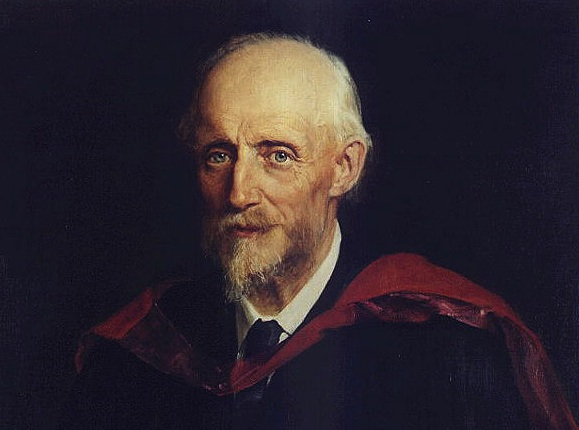
\includegraphics[height=47mm]{osbourne_reynolds1904_crop.jpg}}
  \put( 65, 0){\color{gris} \small \rm Tableau de J. Collierde (1904)}
  \put( 65, 6){\color{gris} \small \rm Osborne REYNOLDS}
  \put( 65, 3){\color{gris} \small \rm (1842 -- 1912)}
\end{picture}

  \vspace{7mm}
  
  \begin{flushright}
    
    \Large
   	\bf
    
    9. Ecoulements en conduite

  \end{flushright}

  \vspace{5mm}

\end{frame}

%%%%%%%%%%%%%%%%%%%%%%%%%%%%%%%%%%%%%%%%%%%%%%%%%%%%%%%%%%%%%%%%%%%%%%%%%%%%%%%%%%%%%%%%%%
% Sommaire :
%%%%%%%%%%%%%%%%%%%%%%%%%%%%%%%%%%%%%%%%%%%%%%%%%%%%%%%%%%%%%%%%%%%%%%%%%%%%%%%%%%%%%%%%%%

\handout{
\begin{frame}{Sommaire}

\small
  
\hspace*{2mm}
\begin{tabular}{cc}
		%&
  		\begin{minipage}{62mm}
  			\tableofcontents[firstsection=-7]
      \vspace{15mm}
  		\end{minipage}
  		&   
  		\begin{minipage}{60cm}
		  \vspace*{-5mm}  
  			%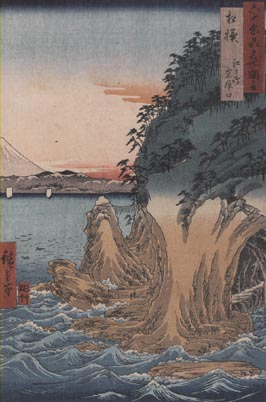
\includegraphics[width=40mm]{vagues.jpg} 
  		\end{minipage}
  	\end{tabular}

\vspace{0mm}

\end{frame}
}

%%%%%%%%%%%%%%%%%%%%%%%%%%%%%%%%%%%%%%%%%%%%%%%%%%%%%%%%%%%%%%%%%%%%%%%%%%%%%%%%%%%%%%%%%%
\section{\bfseries Ecoulements en conduite}
%%%%%%%%%%%%%%%%%%%%%%%%%%%%%%%%%%%%%%%%%%%%%%%%%%%%%%%%%%%%%%%%%%%%%%%%%%%%%%%%%%%%%%%%%%

%==========================================================================================
\subsection{Phénoménologie -- Observations}
%=========================================================================================

%-----------------------------------------------------------------------------------------
\subsubsection{Expérience de Reynolds}
%-----------------------------------------------------------------------------------------
\begin{frame}{Expérience de Reynolds (1883)}
%-----------------------------------------------------------------------------------------

\small

\begin{center}
	\begin{picture}(122, 62)(5, -5)
		\put(0, 0){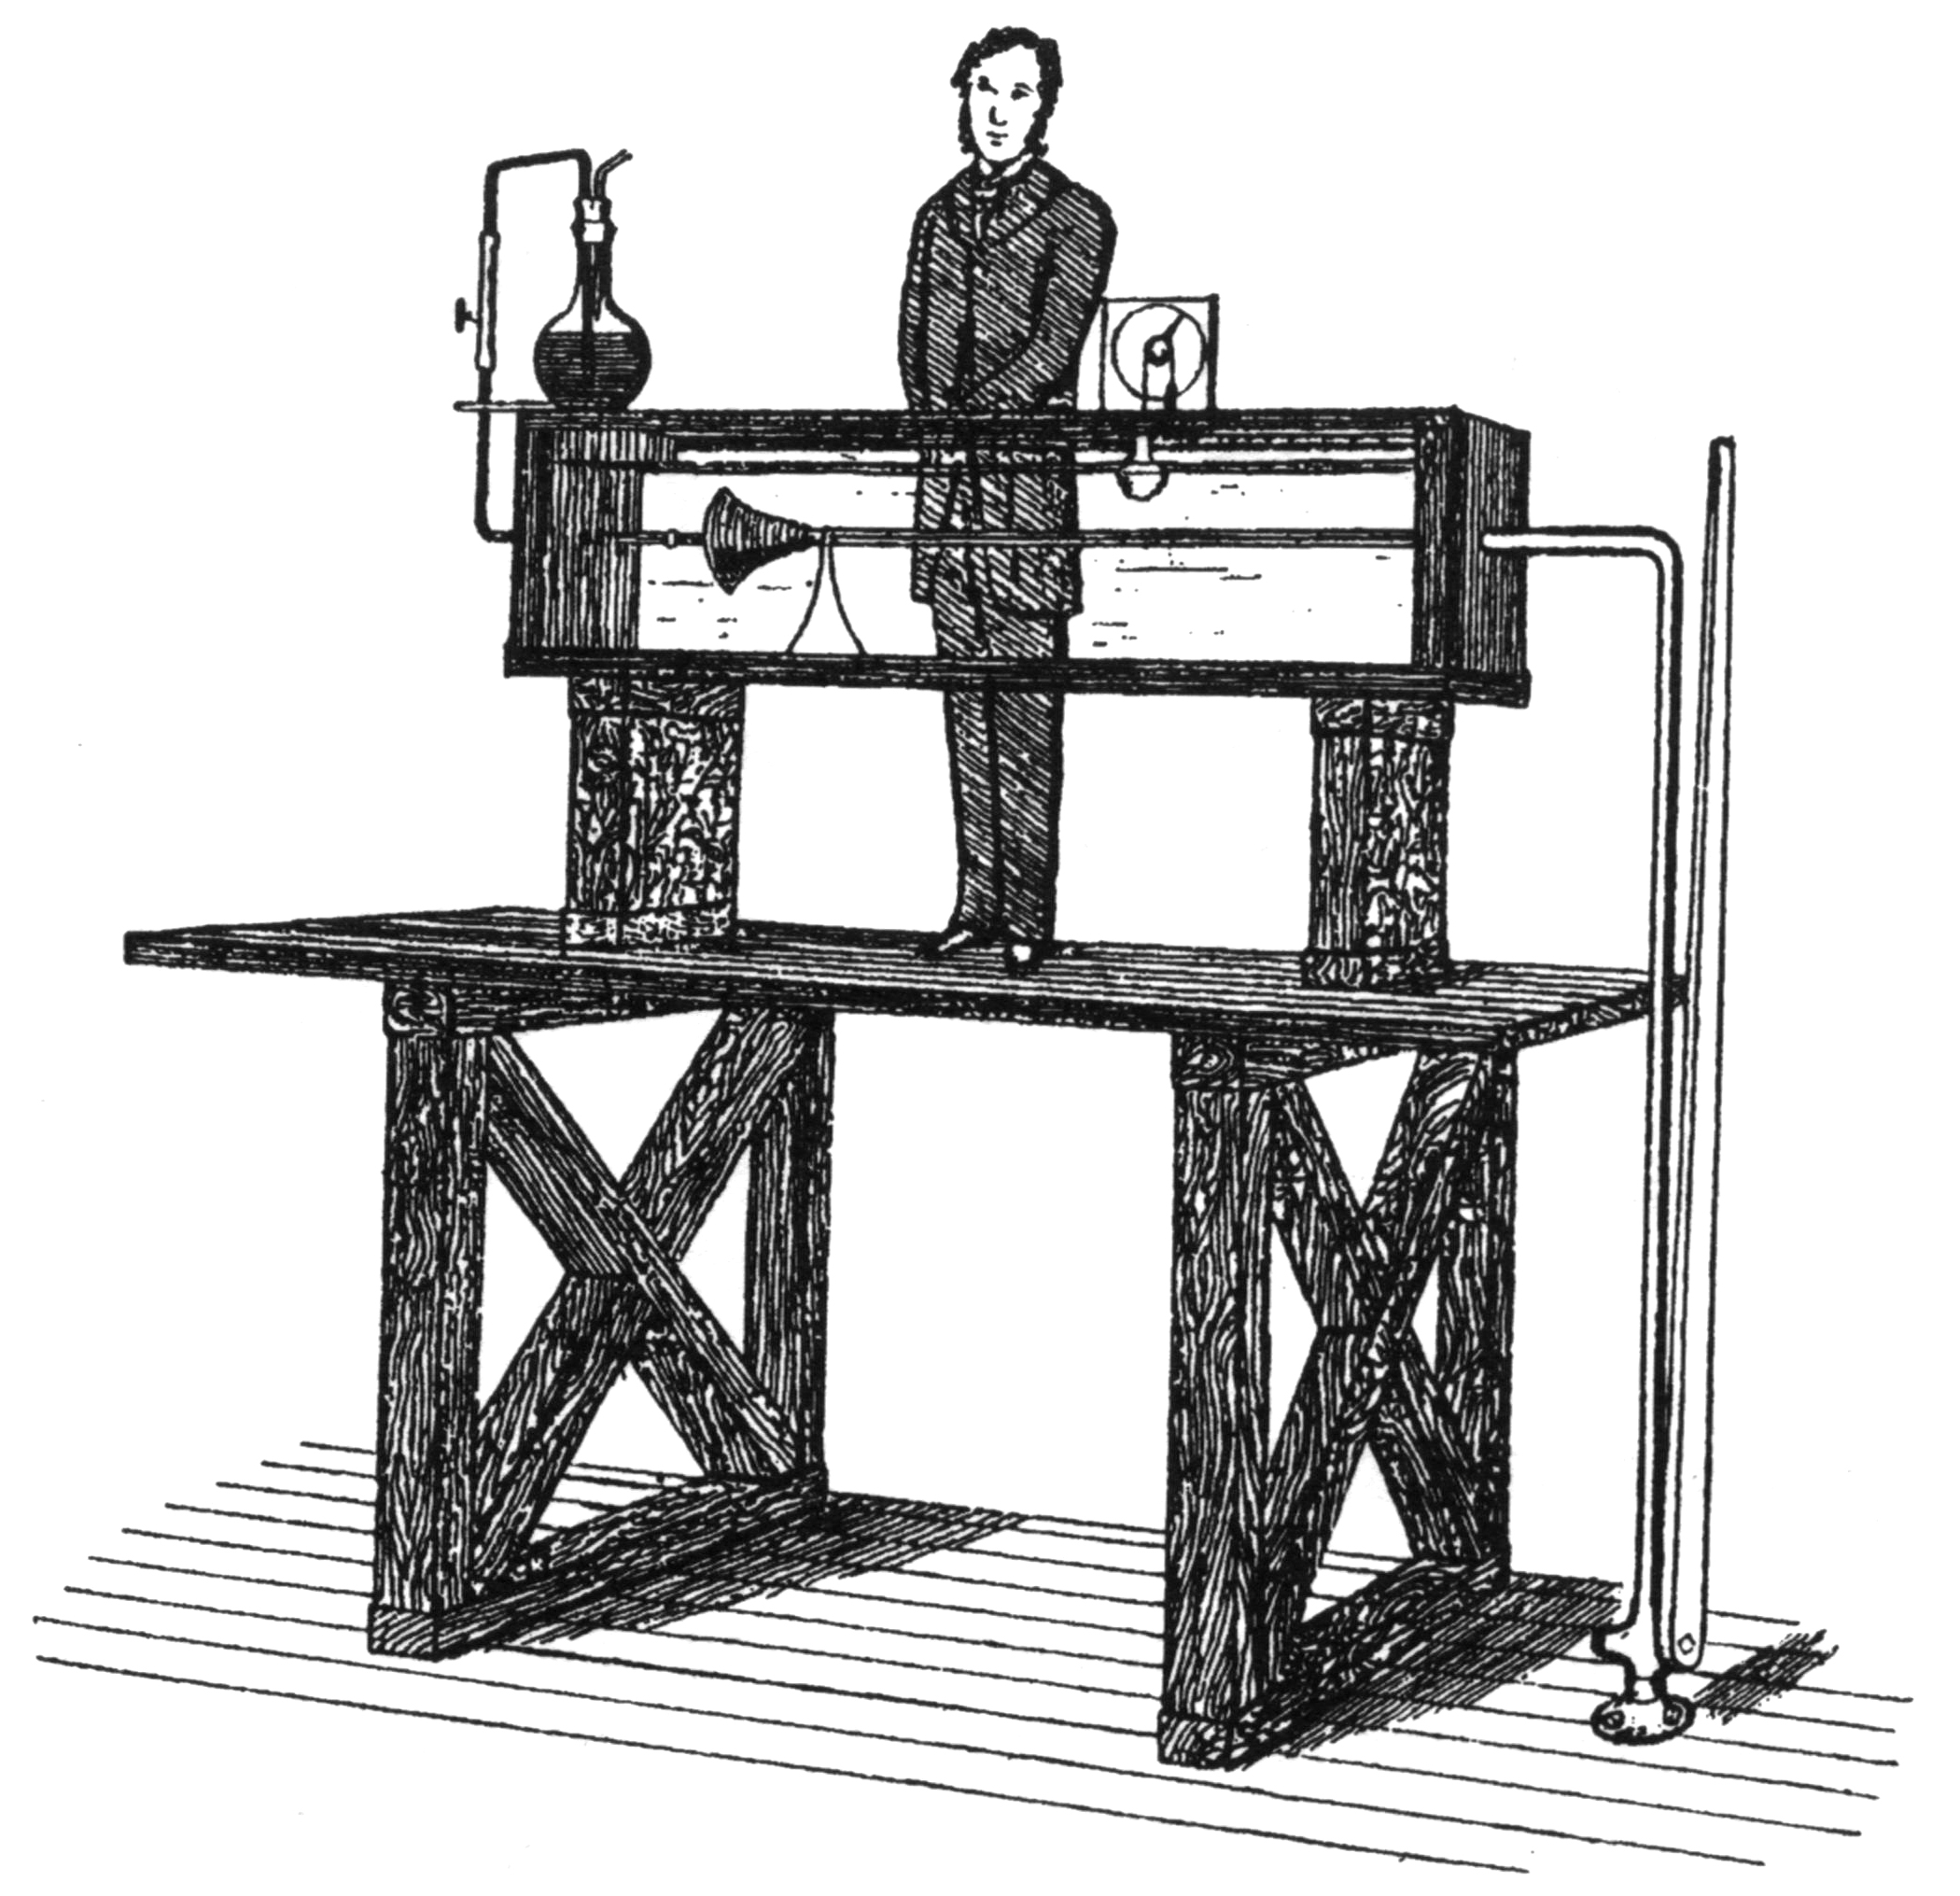
\includegraphics[width=60mm]{Reynolds_fluid_turbulence_experiment_1883.jpg}}
		\put(60, 18){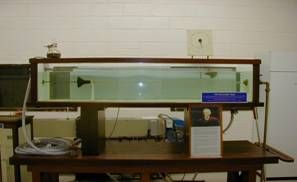
\includegraphics[width=50mm]{manip_Reynolds_photo.jpg}}
		\put(61, 12){Banc expérimental utilisé par Reynolds,}
		\put(61, 9){exposé à l'Université de Manchester (UK)}
	\end{picture}
\end{center}

\vspace{0mm}

\end{frame}

%-----------------------------------------------------------------------------------------
\begin{frame}{Principe de l'expérience}
%-----------------------------------------------------------------------------------------

\small


\begin{center}
	\begin{picture}(97, 15)
		\put(7, 13){\color{rouge} \vector(0, -1){3}}
		\put(10, 10){\color{rouge} injection de colorant}
		\put(7, 0){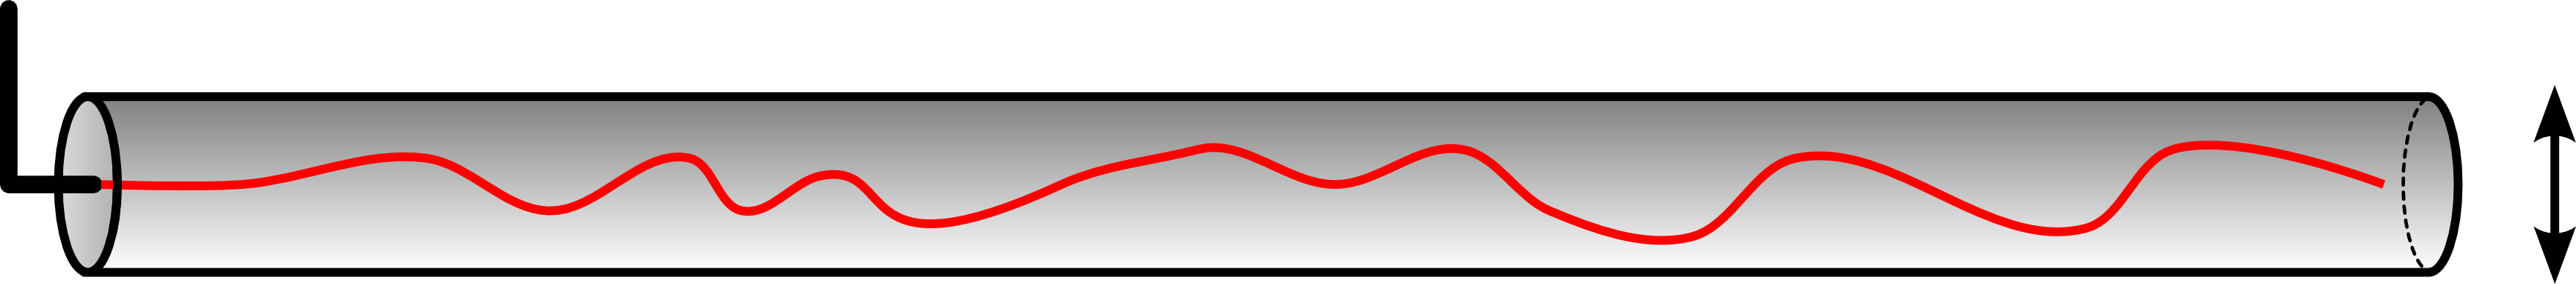
\includegraphics[width=80mm]{principe_experience_Reynolds.png}}
		\put(88, 2.5){$D=2R$}
		\put(0, 3){\color{bleu} \vector(1, 0){5}}
		\put(1, 4.5){\color{bleu} $U$}
		\put(0, 0){\color{bleu} $\rho, \nu$}
	\end{picture}
\end{center}

\smallskip \pause \qquad  {\color{bleu} ($U = \dot m / (\rho \pi R^2)$ vitesse moyenne ou vitesse débitante, déduite du débit-masse $\dot m$)}

\bigskip \pause


Un unique \textsl{paramètre sans dimension} : 

\begin{center}
$\color{rouge}\displaystyle Re = \frac{UD}{\nu} =  \frac{4 \dot m }{\pi \mu D}$
\quad (nombre de Reynolds)  
\end{center}

\medskip \pause

\textbf{Constat de O. Reynolds :} 

\medskip
Les expériences effectuées pour différentes valeurs de $U$, $D$, $\rho$ et $\nu$
montrent que les écoulements observés sont 
\textcolor{rouge}{similaires si le nombre de Reynolds est le même.}

\pause

\medskip
Ce nombre sans dimension joue ainsi le rôle de \textcolor{vert}{paramètre de contrôle}, 
qui permet de déterminer le régime d'écoulement observé.


\vspace{10mm}

\end{frame}

%-----------------------------------------------------------------------------------------
\begin{frame}{Observations expérimentales}
%-----------------------------------------------------------------------------------------

\small

%\vspace{-5mm}
%\hfill Nombre de Reynolds \quad $\color{rouge}\displaystyle Re = \frac{UD}{\nu} = \rho \frac{UD}{\mu}$

%\bigskip

Reynolds observe schématiquement trois régimes distincts :

\begin{picture}(0, 0)(-70, -2.8)
	\put(0, 0){\movie[width=10mm,poster,externalviewer,showcontrols=false]{\colorbox{bleu}{\color{white}visualisations}}{./Figures/Reynolds_experiment.mp4}}
\end{picture}

\pause

\begin{itemize}[<+-| alert@+>]
\item[]
\begin{picture}(100, 17)
	\put(-6, 12){$Re \mylesssim 2000$ : régime laminaire}  
	\put(65, 4.5){%
		\begin{minipage}{40mm} 
			écoulement stationnaire, \\ axisymétrique, établi, 1D \\ (écoulement de Poiseuille)
		\end{minipage}}
	\put(0, 0){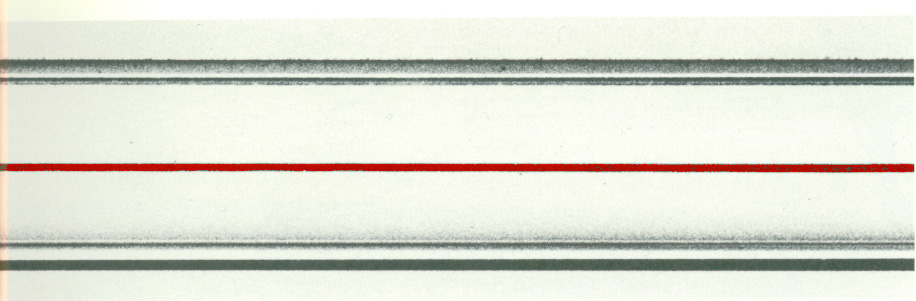
\includegraphics[width=60mm, height=10mm]{Reynolds_laminar_colorized.jpg}}
\end{picture}
\item[]
\begin{picture}(100, 19)
	\put(-6, 12){$2000 \mylesssim Re \mylesssim 4000$ : régime de transition}  
	\put(65, 5){%
		\begin{minipage}{50mm} 
			écoulement instationnaire, \\ 3D par intermittence, \\ sinon relaminarisation
		\end{minipage}}
	\put(0, 0){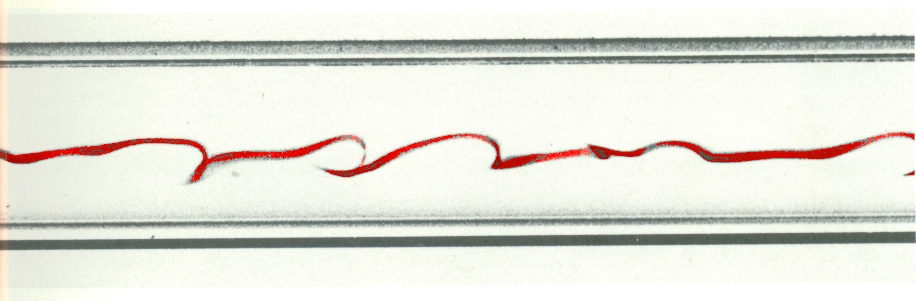
\includegraphics[width=60mm, height=10mm]{Reynolds_transition_colorized.jpg}}
\end{picture}
\item[]
\begin{picture}(100, 19)
	\put(-6, 12){$4000 \mylesssim Re$ : régime turbulent}  
	\put(65, 4.5){%
		\begin{minipage}{50mm} 
			écoulement très instationnaire, \\ fortement 3D, "chaotique" \\ petits et gros tourbillons
		\end{minipage}}
	\put(0, 0){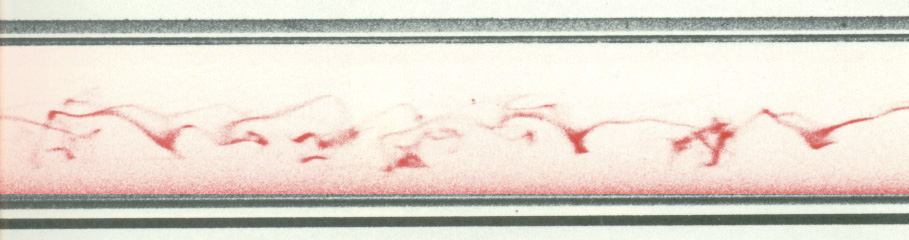
\includegraphics[width=60mm, height=10mm]{Reynolds_turbulent_colorized.jpg}}
\end{picture}
\end{itemize}

\vspace{0mm}

\end{frame}

%-----------------------------------------------------------------------------------------
\subsubsection{Régime laminaire}
%-----------------------------------------------------------------------------------------
\begin{frame}{Régime laminaire $Re \mylesssim 2000$}
%-----------------------------------------------------------------------------------------

\small

Pour $Re \mylesssim 2000$, Reynolds observe le régime dit \textcolor{vert}{laminaire}
pour lequel l'écoulement est 
stationnaire, axisymétrique, établi, 1D : l'expérience montre qu'il s'agit de l'écoulement de \textcolor{vert}{Poiseuille}, 
dont le champ de vitesse est donné par 

\[
	u(r) = -\frac{R^2}{4\mu} \frac{dp}{dx} \, \left( 1 - \frac{r^2}{R^2} \right ) 
	  %   = 2 U \, \left( 1 - \frac{r^2}{R^2} \right )
\]
$$
U = \frac{u_{max}}{2} = \frac{R^2}{8\mu} \left| \frac{dp}{dx} \right| 
$$

\begin{center}
	\begin{picture}(95, 22)
		\put(0, 0){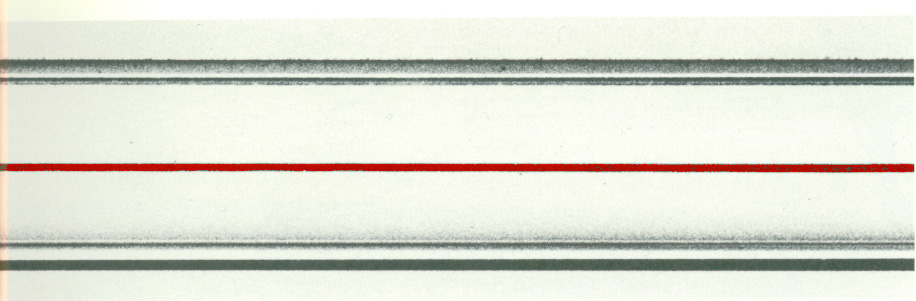
\includegraphics[width=50mm, height=20mm]{Reynolds_laminar_colorized.jpg}}
		\put(55, 0){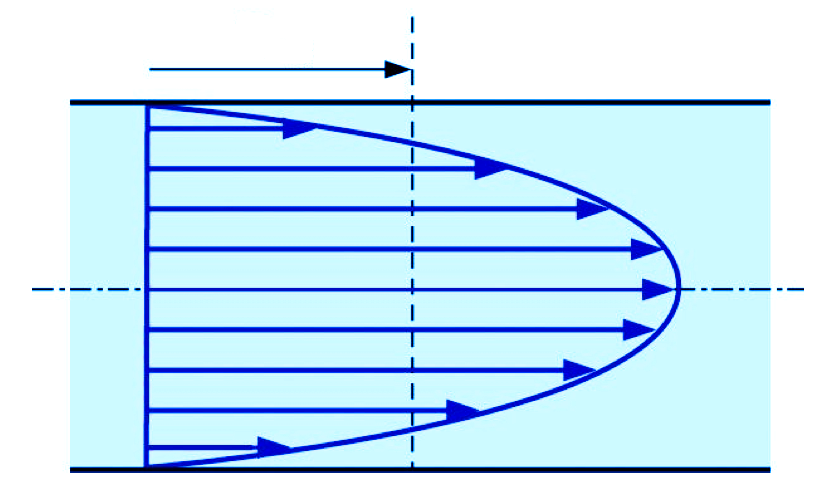
\includegraphics[width=40mm]{poiseuille.png}}
		\put(86, 15){\color{bleu} $u(r)$}
		\put(76, 20){\color{bleu} $U$}
	\end{picture}
\end{center}

\pause

Le profil de vitesse parabolique correspondant à l'écoulement de Poiseuille est \textcolor{vert}{une solution exacte} de
l'équation de Navier--Stokes quelle que soit la valeur du nombre de Reynolds.

\medskip

En général, cet écoulement se déstabilise pour $Re \sim 2000$, 
au delà apparaît \textcolor{vert}{une autre solution}
de l'équation de Navier--Stokes, plus compliquée, dont on ne connaît pas l'expression mathématique\ldots

\medskip

Cependant, dans des conditions très "propres" (perturbations en entrée très faibles, et tube est très lisse), la solution de Poiseuille peut être observée jusqu'à des nombres de Reynolds de l'ordre de $10^5$ !


(pour $Re>2000$ La solution laminaire est donc \textcolor{red}{métastable}...)


\vspace{0mm}

\end{frame}

%-----------------------------------------------------------------------------------------
\subsubsection{Régime de transition}
%-----------------------------------------------------------------------------------------
\begin{frame}{Régime de transition $2000 \mylesssim Re \mylesssim 4000$}
%-----------------------------------------------------------------------------------------

\small

Pour les nombres de Reynolds intermédiaires, compris entre 2000 et 4000 environ (dans des conditions ordinaires), 
on observe un régime dit \textcolor{vert}{transitoire} ou de transition : "bouffées" de turbulence (écoulement instationnaire et 3D), alternant avec des 
phases de relaminarisation.


\begin{center}
	\begin{picture}(60, 12)
		\put(0, 0){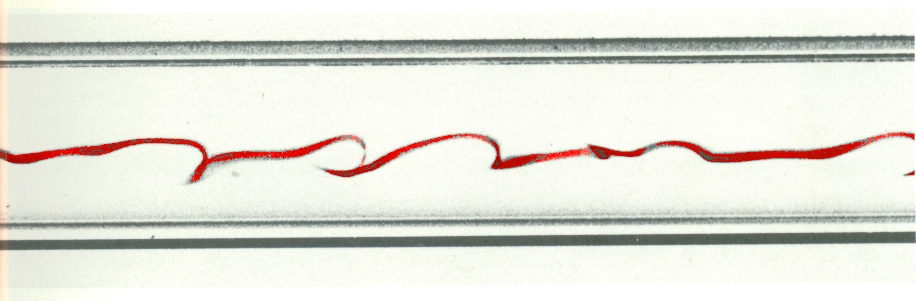
\includegraphics[width=60mm, height=10mm]{Reynolds_transition_colorized.jpg}}
	\end{picture}
\end{center}

\pause

\bigskip

Ce régime est le plus complexe à décrire et à comprendre : il fait l'objet
de nombreuses recherches actuelles, aussi bien par le biais de \textcolor{vert}{campagnes expérimentales}
que de \textcolor{vert}{simulations numériques} et d'\textcolor{vert}{analyses théoriques}. 

\medskip


%Ainsi, si le niveau des perturbations en entrée est très faible, et si le tube est très lisse, cet écoulement peut être observé
%jusqu'à des nombres de Reynolds de l'ordre de $10^5$ !


Les concepts adaptés à l'étude de ce régime de transition proviennent de
\begin{itemize}
	\item[\checkmark] la théorie des instabilités hydrodynamiques
	\item[\checkmark] la théorie des systèmes dynamiques non linéaires
	\item[\checkmark] la théorie des bifurcations
%	\item[\checkmark] la théorie du contrôle
	\item[\checkmark] [\mbox{\ldots}]
\end{itemize}

\vspace{5mm}

\end{frame}

%-----------------------------------------------------------------------------------------
\subsubsection{Régime turbulent}
%-----------------------------------------------------------------------------------------
\begin{frame}{Régime turbulent $4000 \mylesssim Re$}
%-----------------------------------------------------------------------------------------

\small

Pour les grands nombres de Reynolds, l'écoulement devient \textcolor{vert}{turbulent}
et rentre dans un régime fortement instationnaire, complètement 3D, présentant une structure
spatiale très compliquée \\
avec petits et grands tourbillons, et un comportement temporel "chaotique".

\begin{center}
	\begin{picture}(60, 12)
		\put(0, 0){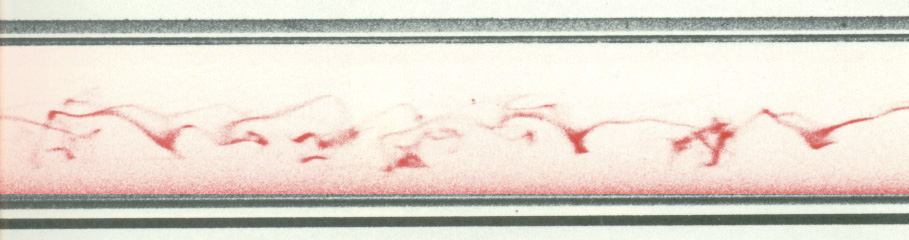
\includegraphics[width=60mm, height=10mm]{Reynolds_turbulent_colorized.jpg}}
	\end{picture}
\end{center}

Paradoxalement, ce régime n'est pas le plus compliqué à modéliser 
si l'on accepte  de se restreindre
aux \textcolor{rouge}{grandeurs moyennes} de l'écoulement
(\textcolor{vert}{approche statistique}).

\pause

\begin{center}
	\begin{picture}(0, 0)(10, -17)
		\put(0, 0){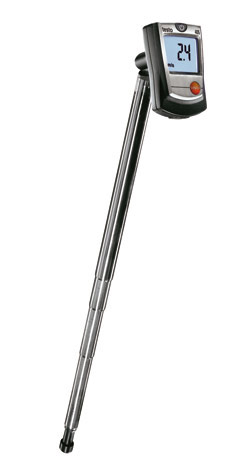
\includegraphics[width=6mm, height=10mm]{testo_405_alpha.png}}
		\put(7, 8){\footnotesize \slshape \color{rouge} sonde de vitesse}
	\end{picture}
\end{center}

\vspace{-3mm}

\color{rouge}{Mesure de vitesse en un point de l'écoulement :}

\begin{overprint}

\onslide<3>

	\begin{picture}(40, 30)(-57, -7)
		\put(0, 0){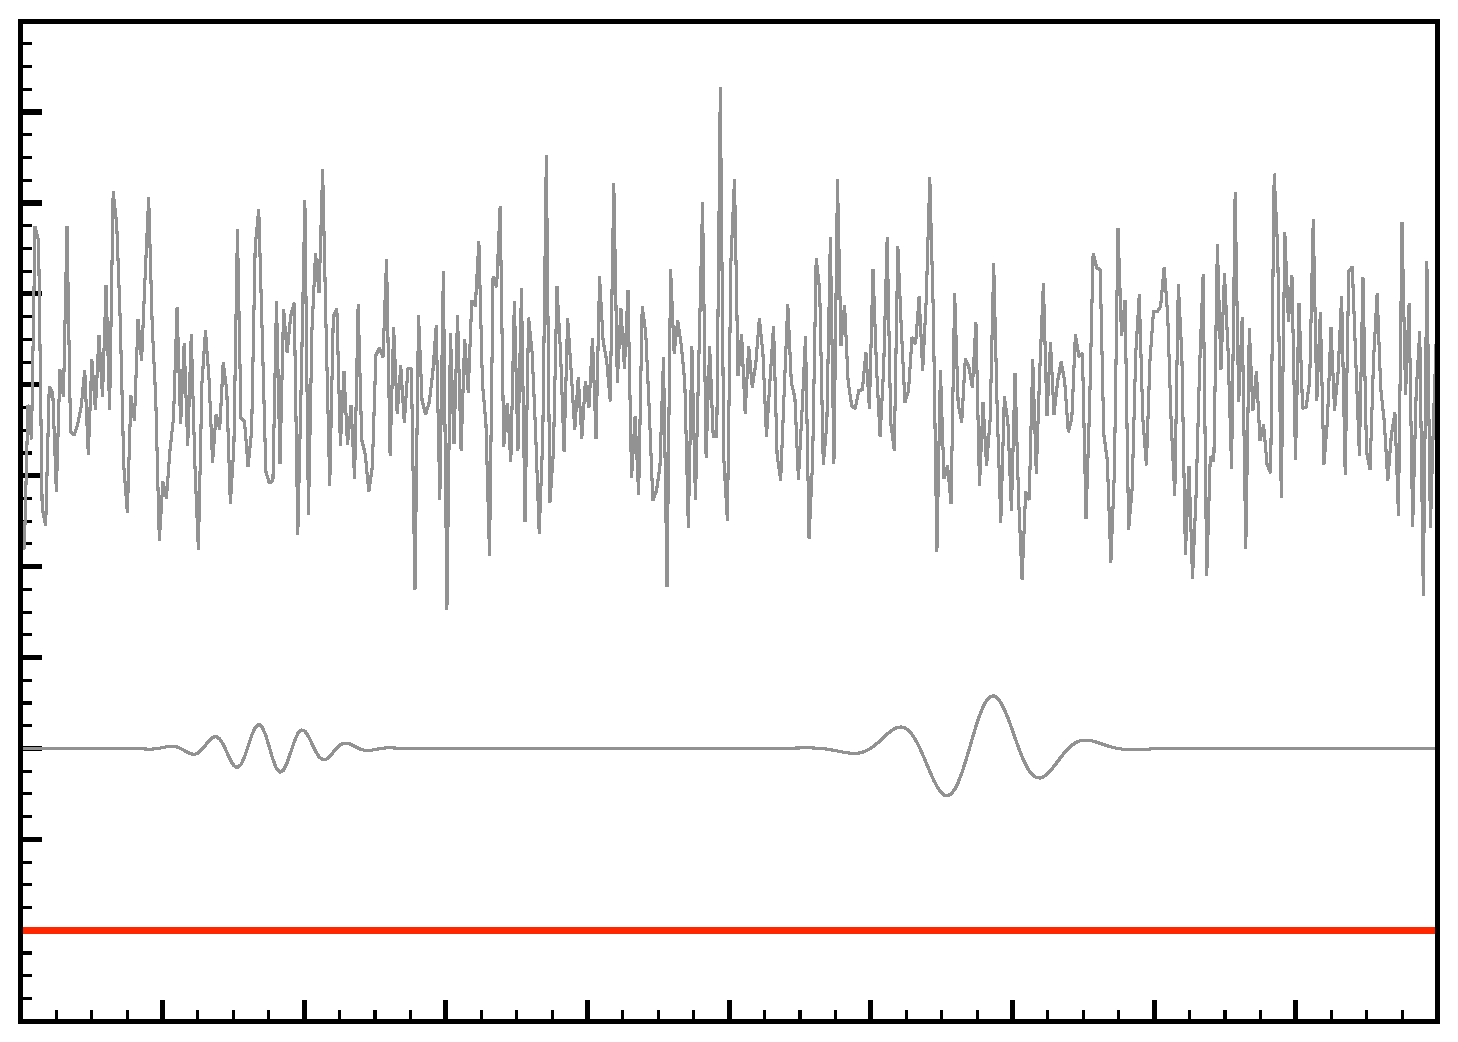
\includegraphics[width=40mm]{plot_laminar.pdf}}
		\put(41, 3){\color{rouge} laminaire}
		\put(20, -3){\color{black} $t$ (s)}
		\put(-6, 15){\color{black} $u(t)$}
		\put(-7, 12){\color{black} (m/s)}
	\end{picture}

\onslide<4>

	\begin{picture}(40, 30)(-57, -7)
		\put(0, 0){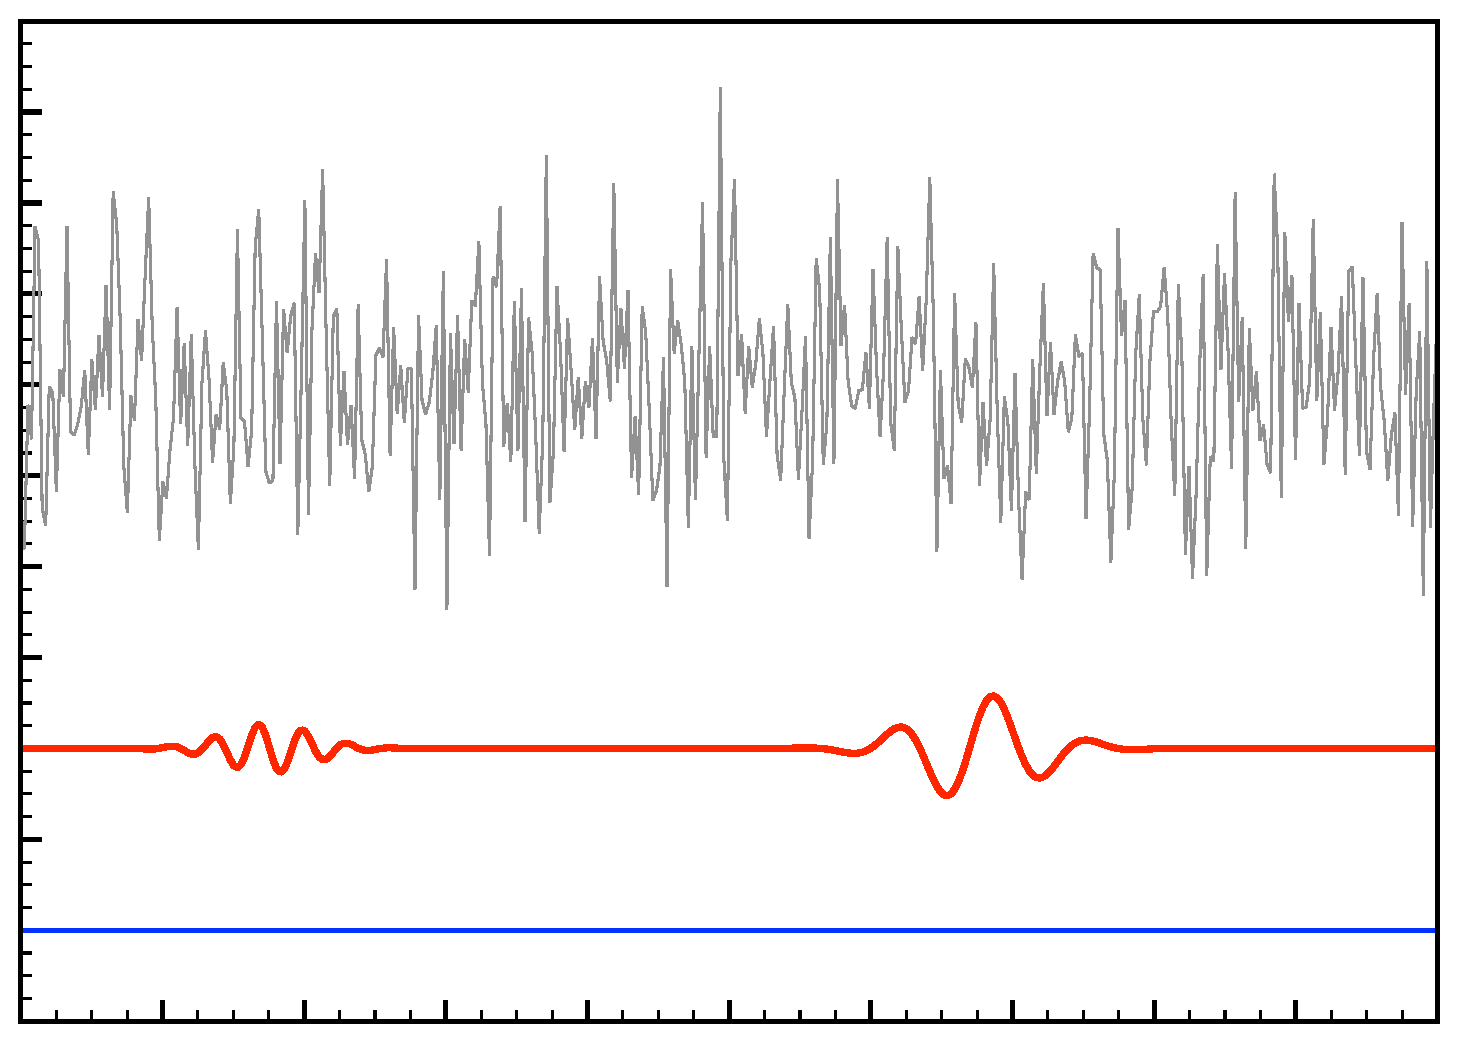
\includegraphics[width=40mm]{plot_transition.pdf}}
		\put(41, 3){\color{bleu} laminaire}
		\put(41, 8){\color{rouge} transition}
		\put(20, -3){\color{black} $t$ (s)}
		\put(-6, 15){\color{black} $u(t)$}
		\put(-7, 12){\color{black} (m/s)}
	\end{picture}

\onslide<5>

	\begin{picture}(40, 30)(-57, -7)
		\put(0, 0){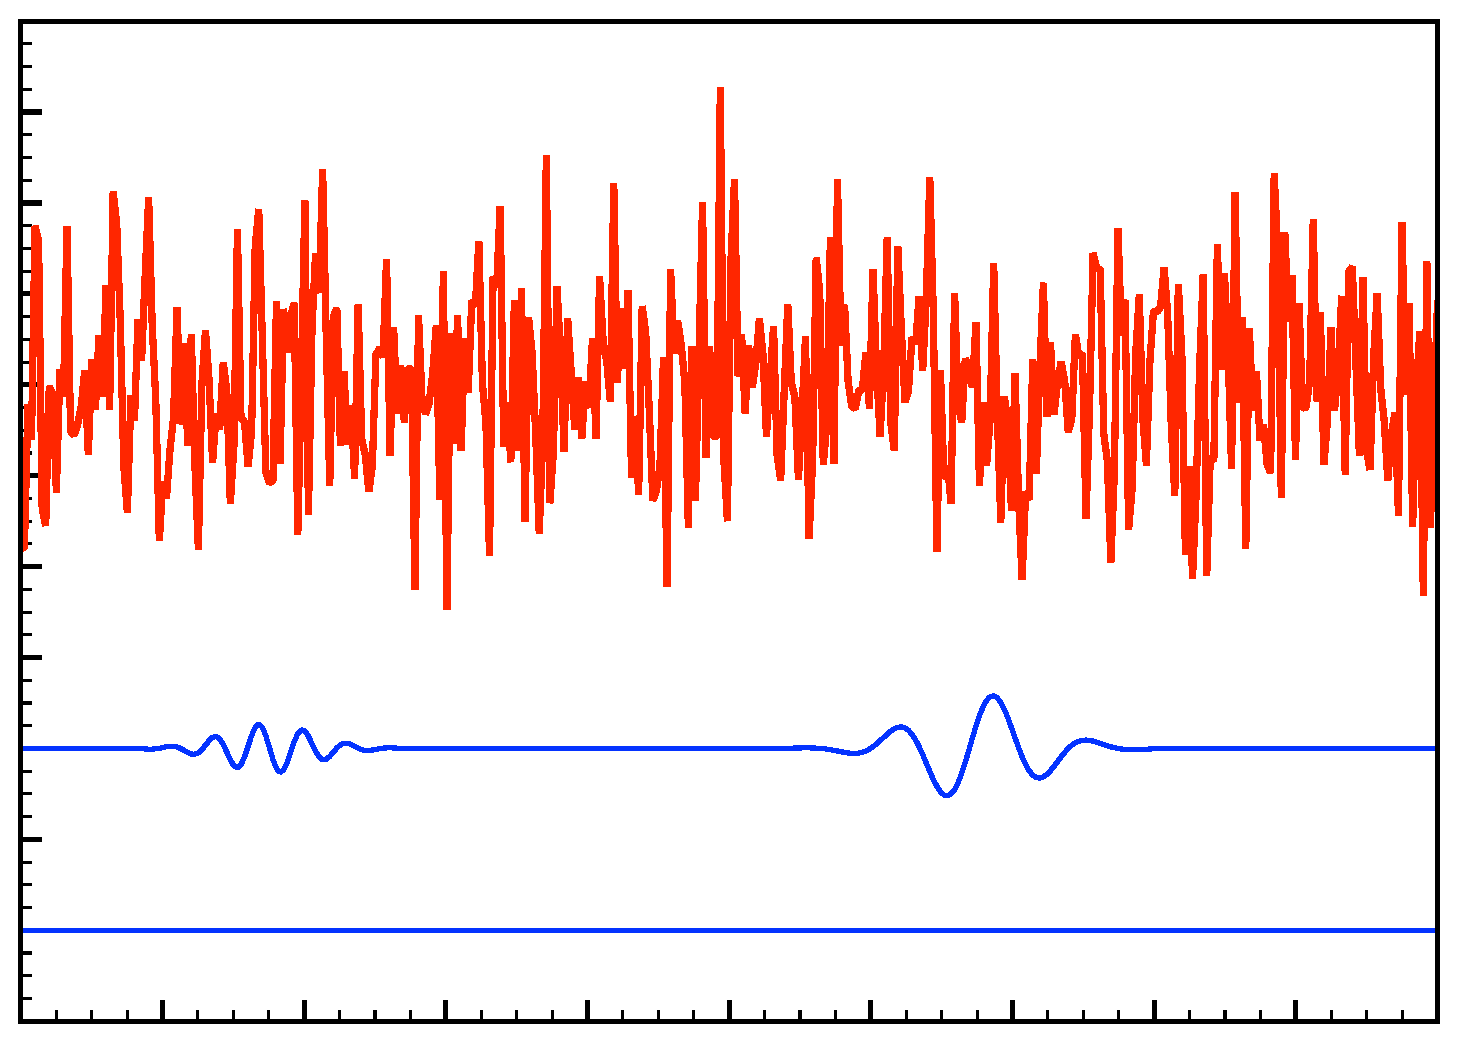
\includegraphics[width=40mm]{plot_turbulent.pdf}}
		\put(41, 3){\color{bleu} laminaire}
		\put(41, 8){\color{bleu} transition}
		\put(41, 18){\color{rouge} turbulent}
		\put(20, -3){\color{black} $t$ (s)}
		\put(-6, 15){\color{black} $u(t)$}
		\put(-7, 12){\color{black} (m/s)}
	\end{picture}

\onslide<6>

	\begin{picture}(40, 30)(-57, -7)
		\put(0, 0){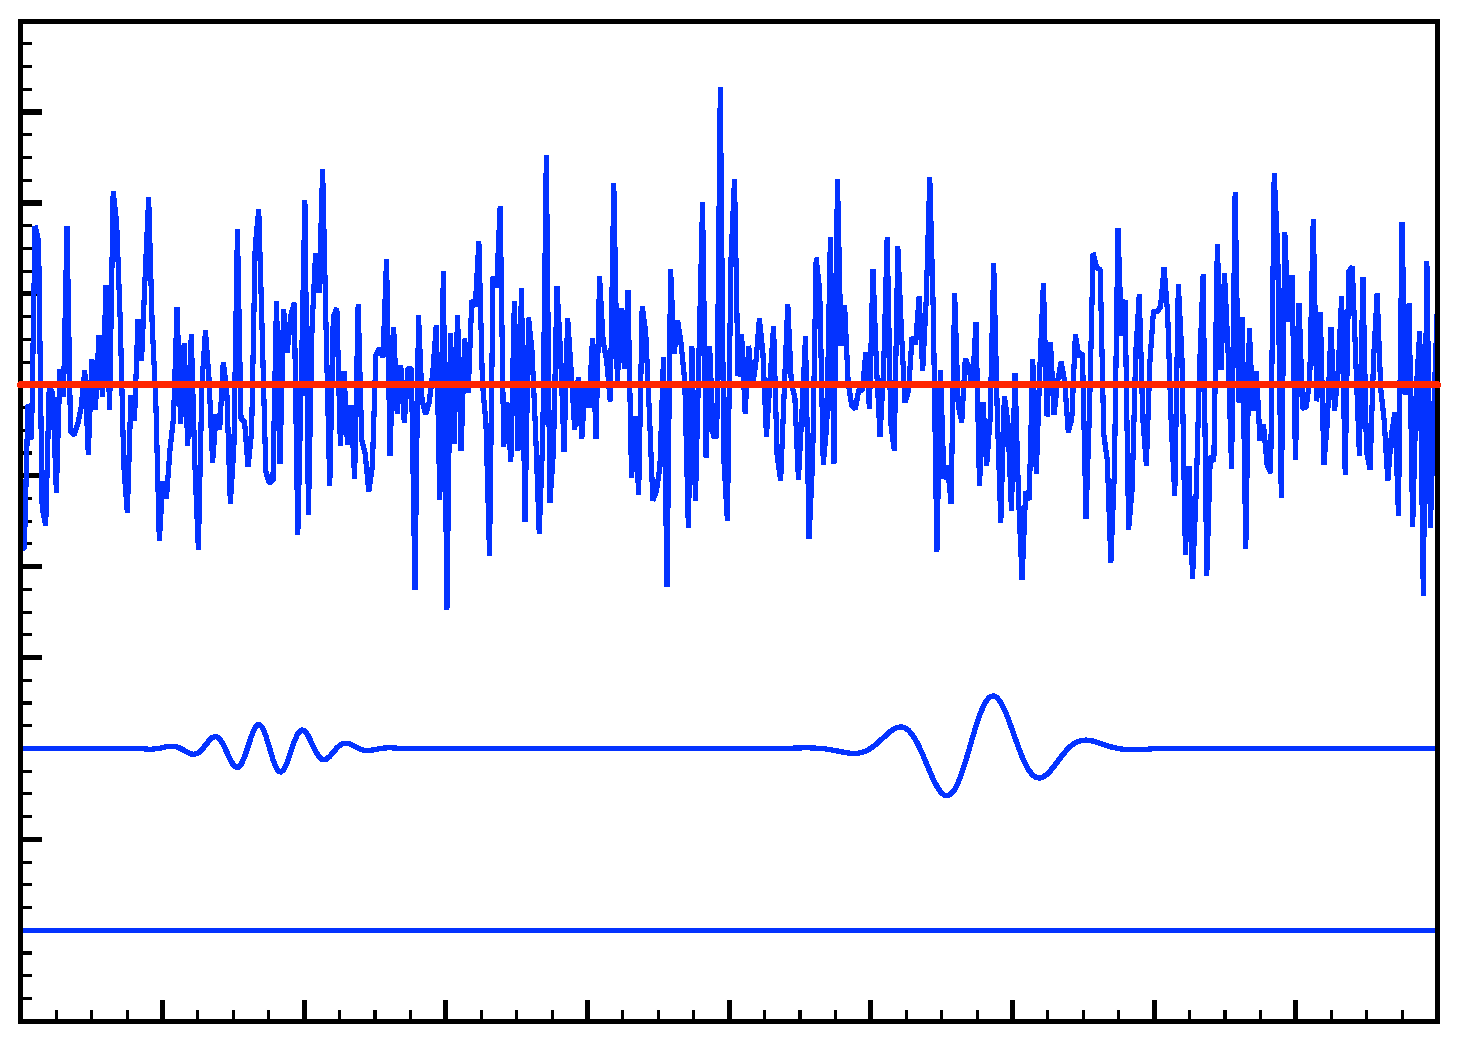
\includegraphics[width=40mm]{plot_turbulent_mean.pdf}}
		\put(41, 3){\color{bleu} laminaire}
		\put(41, 8){\color{bleu} transition}
		\put(41, 18){\color{bleu} turbulent}
		\put(20, -3){\color{black} $t$ (s)}
		\put(-6, 15){\color{black} $u(t)$}
		\put(-7, 12){\color{black} (m/s)}
		\put(0, 18){\color{rouge} \vector(-1, 0){10}}
		\put(-49, 17.5){\color{rouge} vitesse moyenne locale $<u>$}
	\end{picture}

\onslide<7>

	\begin{picture}(40, 30)(-57, -7)
		\put(0, 0){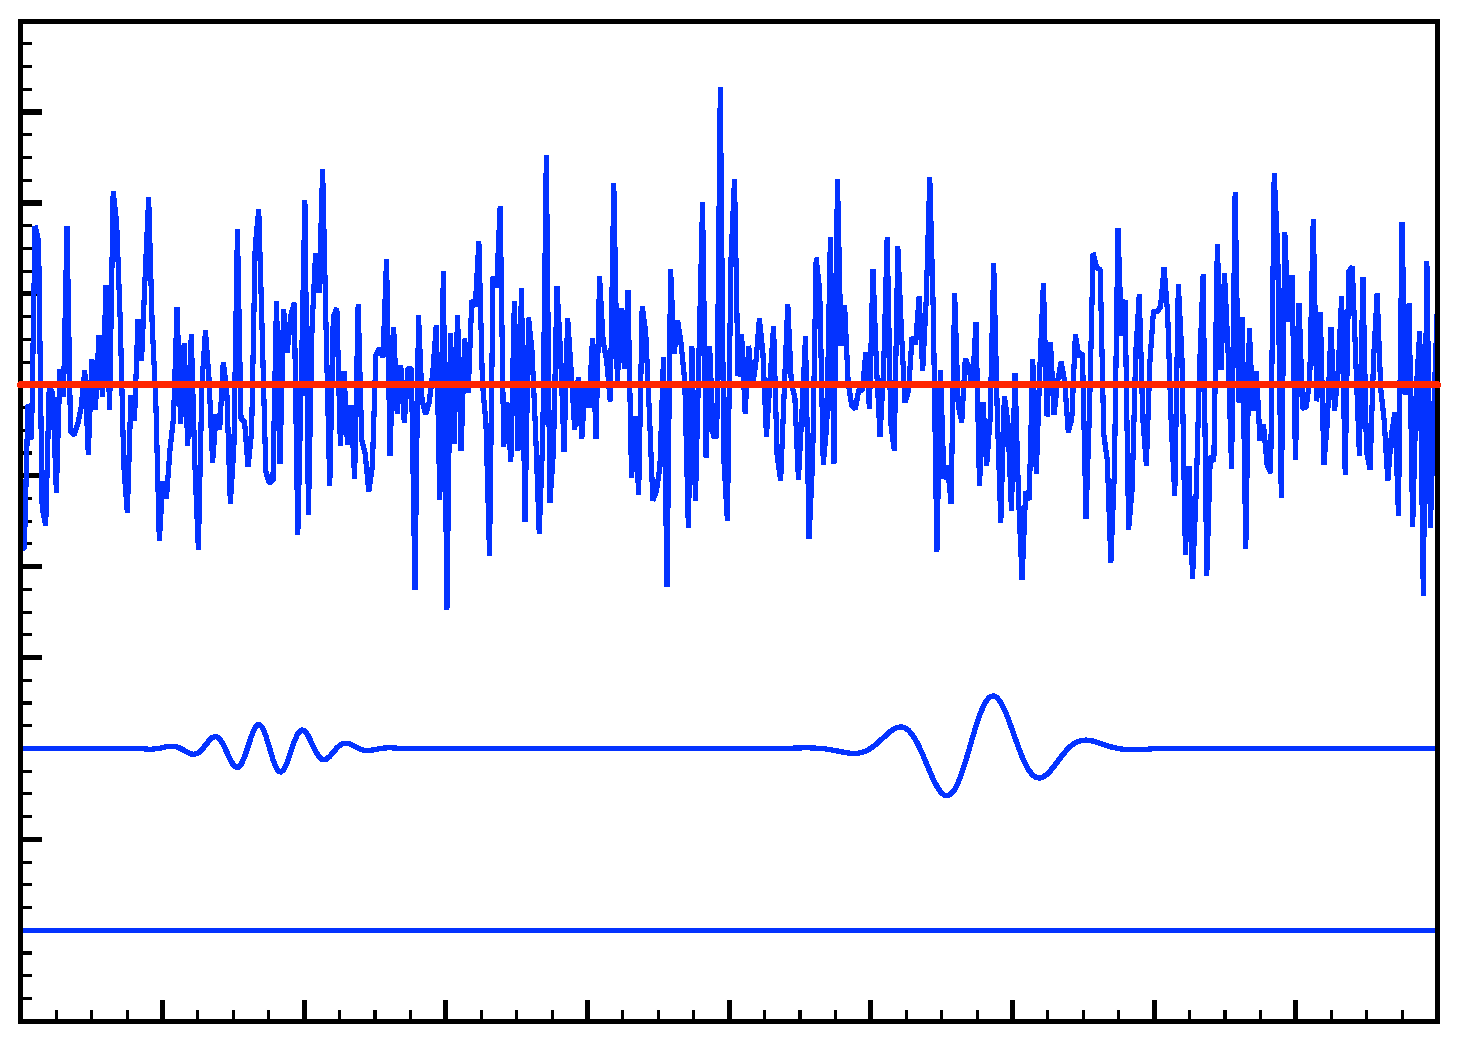
\includegraphics[width=40mm]{plot_turbulent_mean.pdf}}
		\put(41, 3){\color{bleu} laminaire}
		\put(41, 8){\color{bleu} transition}
		\put(41, 18){\color{bleu} turbulent}
		\put(20, -3){\color{black} $t$ (s)}
		\put(-6, 15){\color{black} $u(t)$}
		\put(-7, 12){\color{black} (m/s)}
		\put(0, 18){\color{rouge} \vector(-1, 0){10}}
		\put(-49, 17.5){\color{bleu} vitesse moyenne locale $<u>$}
	\end{picture}

	\begin{picture}(0, 0)(-7, -7)
		\put(0, 0){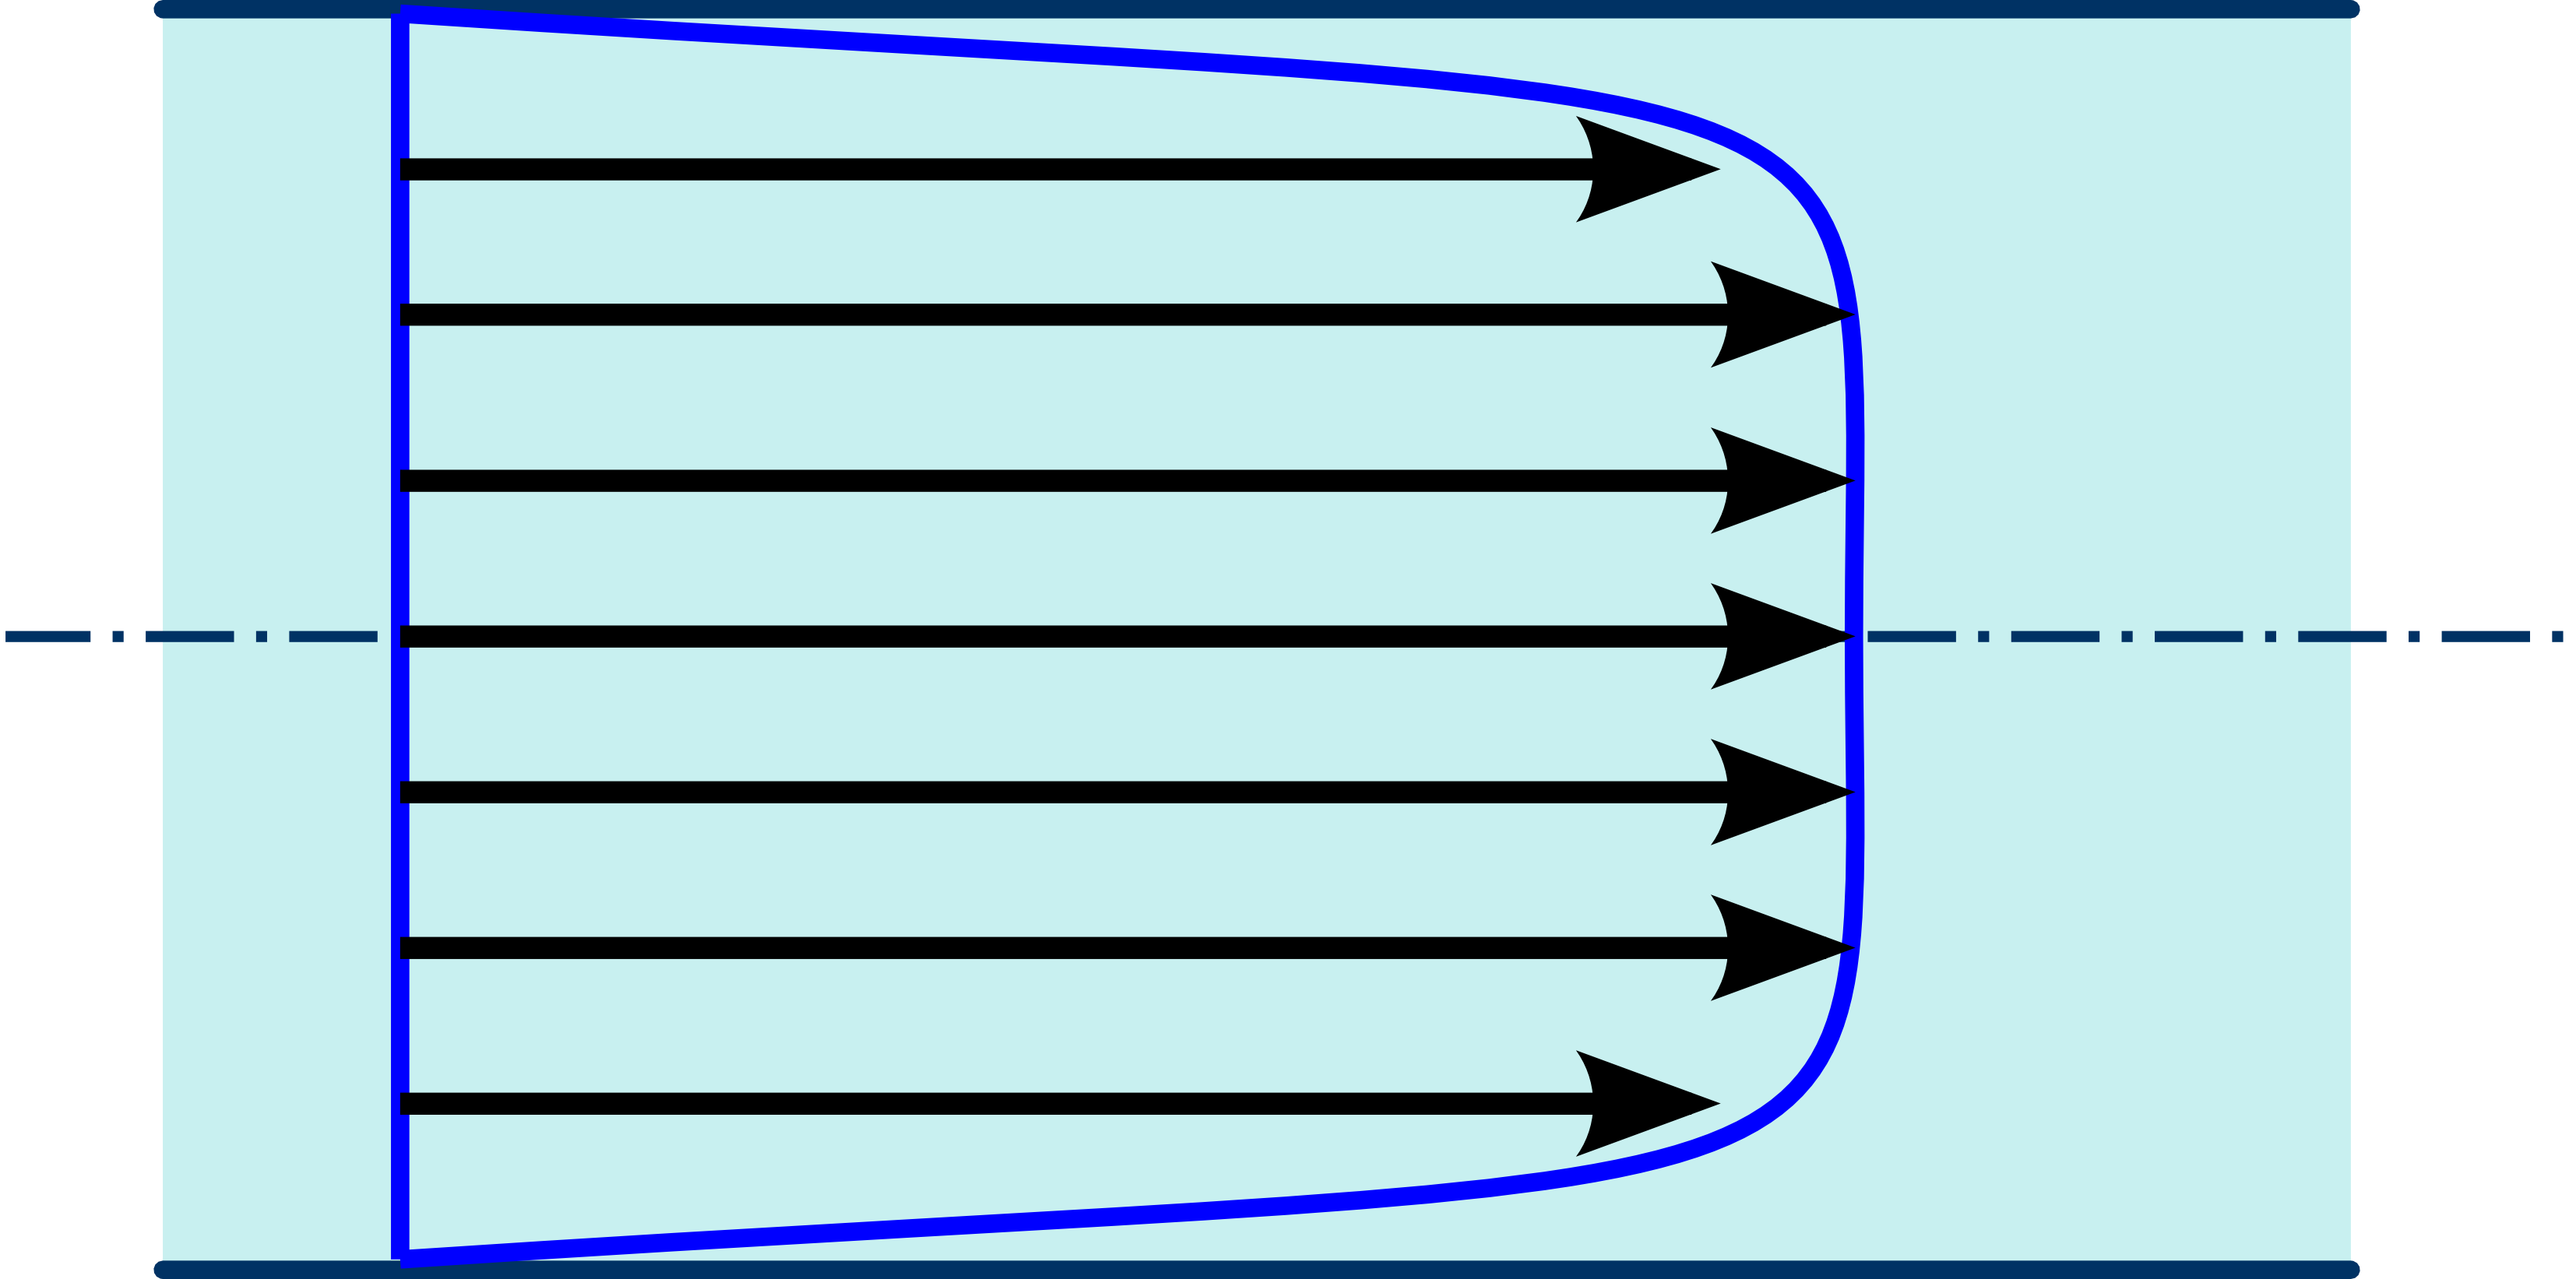
\includegraphics[width=35mm]{profil_turbulent_moyen.png}}
		\put(-2, -4){\color{bleu} Profil de vitesse moyenne (quasi uniforme)}
	\end{picture}



\end{overprint}

\vspace{0mm}

\end{frame}

%==========================================================================================
\subsection{Modélisation et application des bilans intégraux}
%=========================================================================================
%
%%-----------------------------------------------------------------------------------------
%\subsubsection{Modèle d'écoulement}
%%-----------------------------------------------------------------------------------------
%\begin{frame}{Modèle d'écoulement}
%%-----------------------------------------------------------------------------------------
%
%\small
%
%\textbf{Hypothèses de base :} fluide homogène et newtonien, écoulement incompressible.
%
%\medskip \pause
%
%\textbf{Modélisation :}
%\begin{itemize}[<+-| alert@+>]
%\item
%	Si écoulement laminaire : pas de problème (solution de Poiseuille)
%\item
%	Si écoulement transitoire : pas de modélisation disponible 
%	
%	(et forte dépendance aux conditions expérimentales)\ldots 
%\item
%	Si écoulement turbulent : modélisation possible en considérant l'écoulement stationnaire \\ et uniforme "en moyenne" 
%\end{itemize}
%
%\pause
%
%\begin{center}
%	\begin{picture}(95, 20)
%		\put(0, 0.5){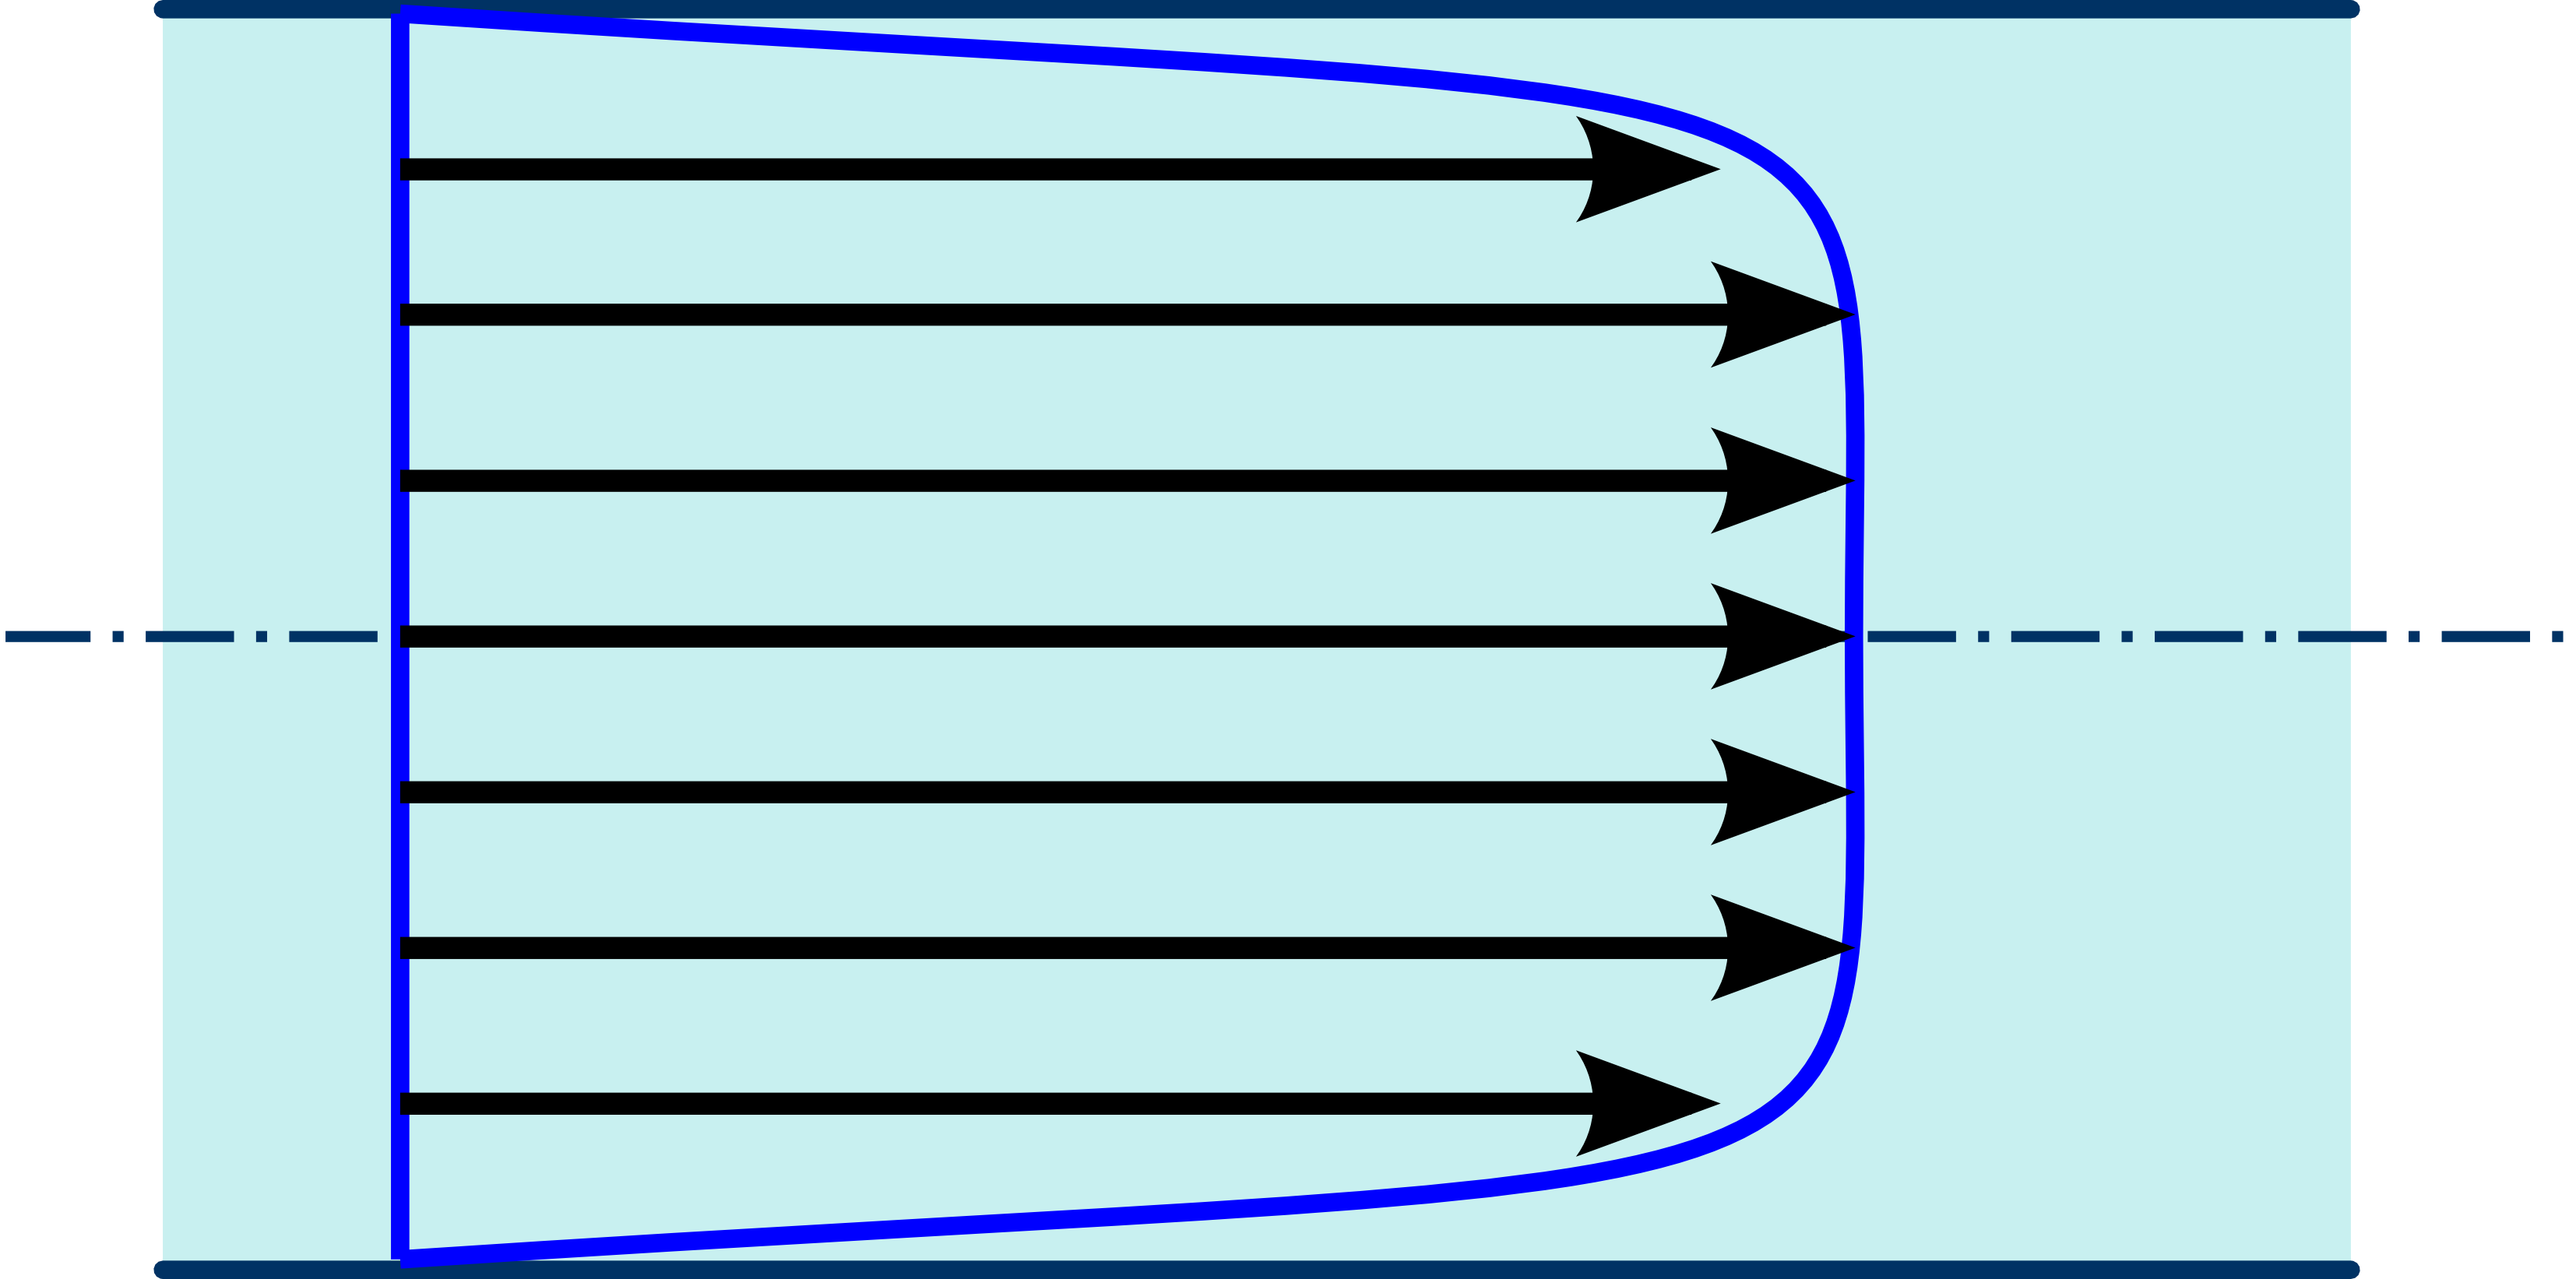
\includegraphics[width=35mm]{profil_turbulent_moyen.png}}
%		\put(60, 0){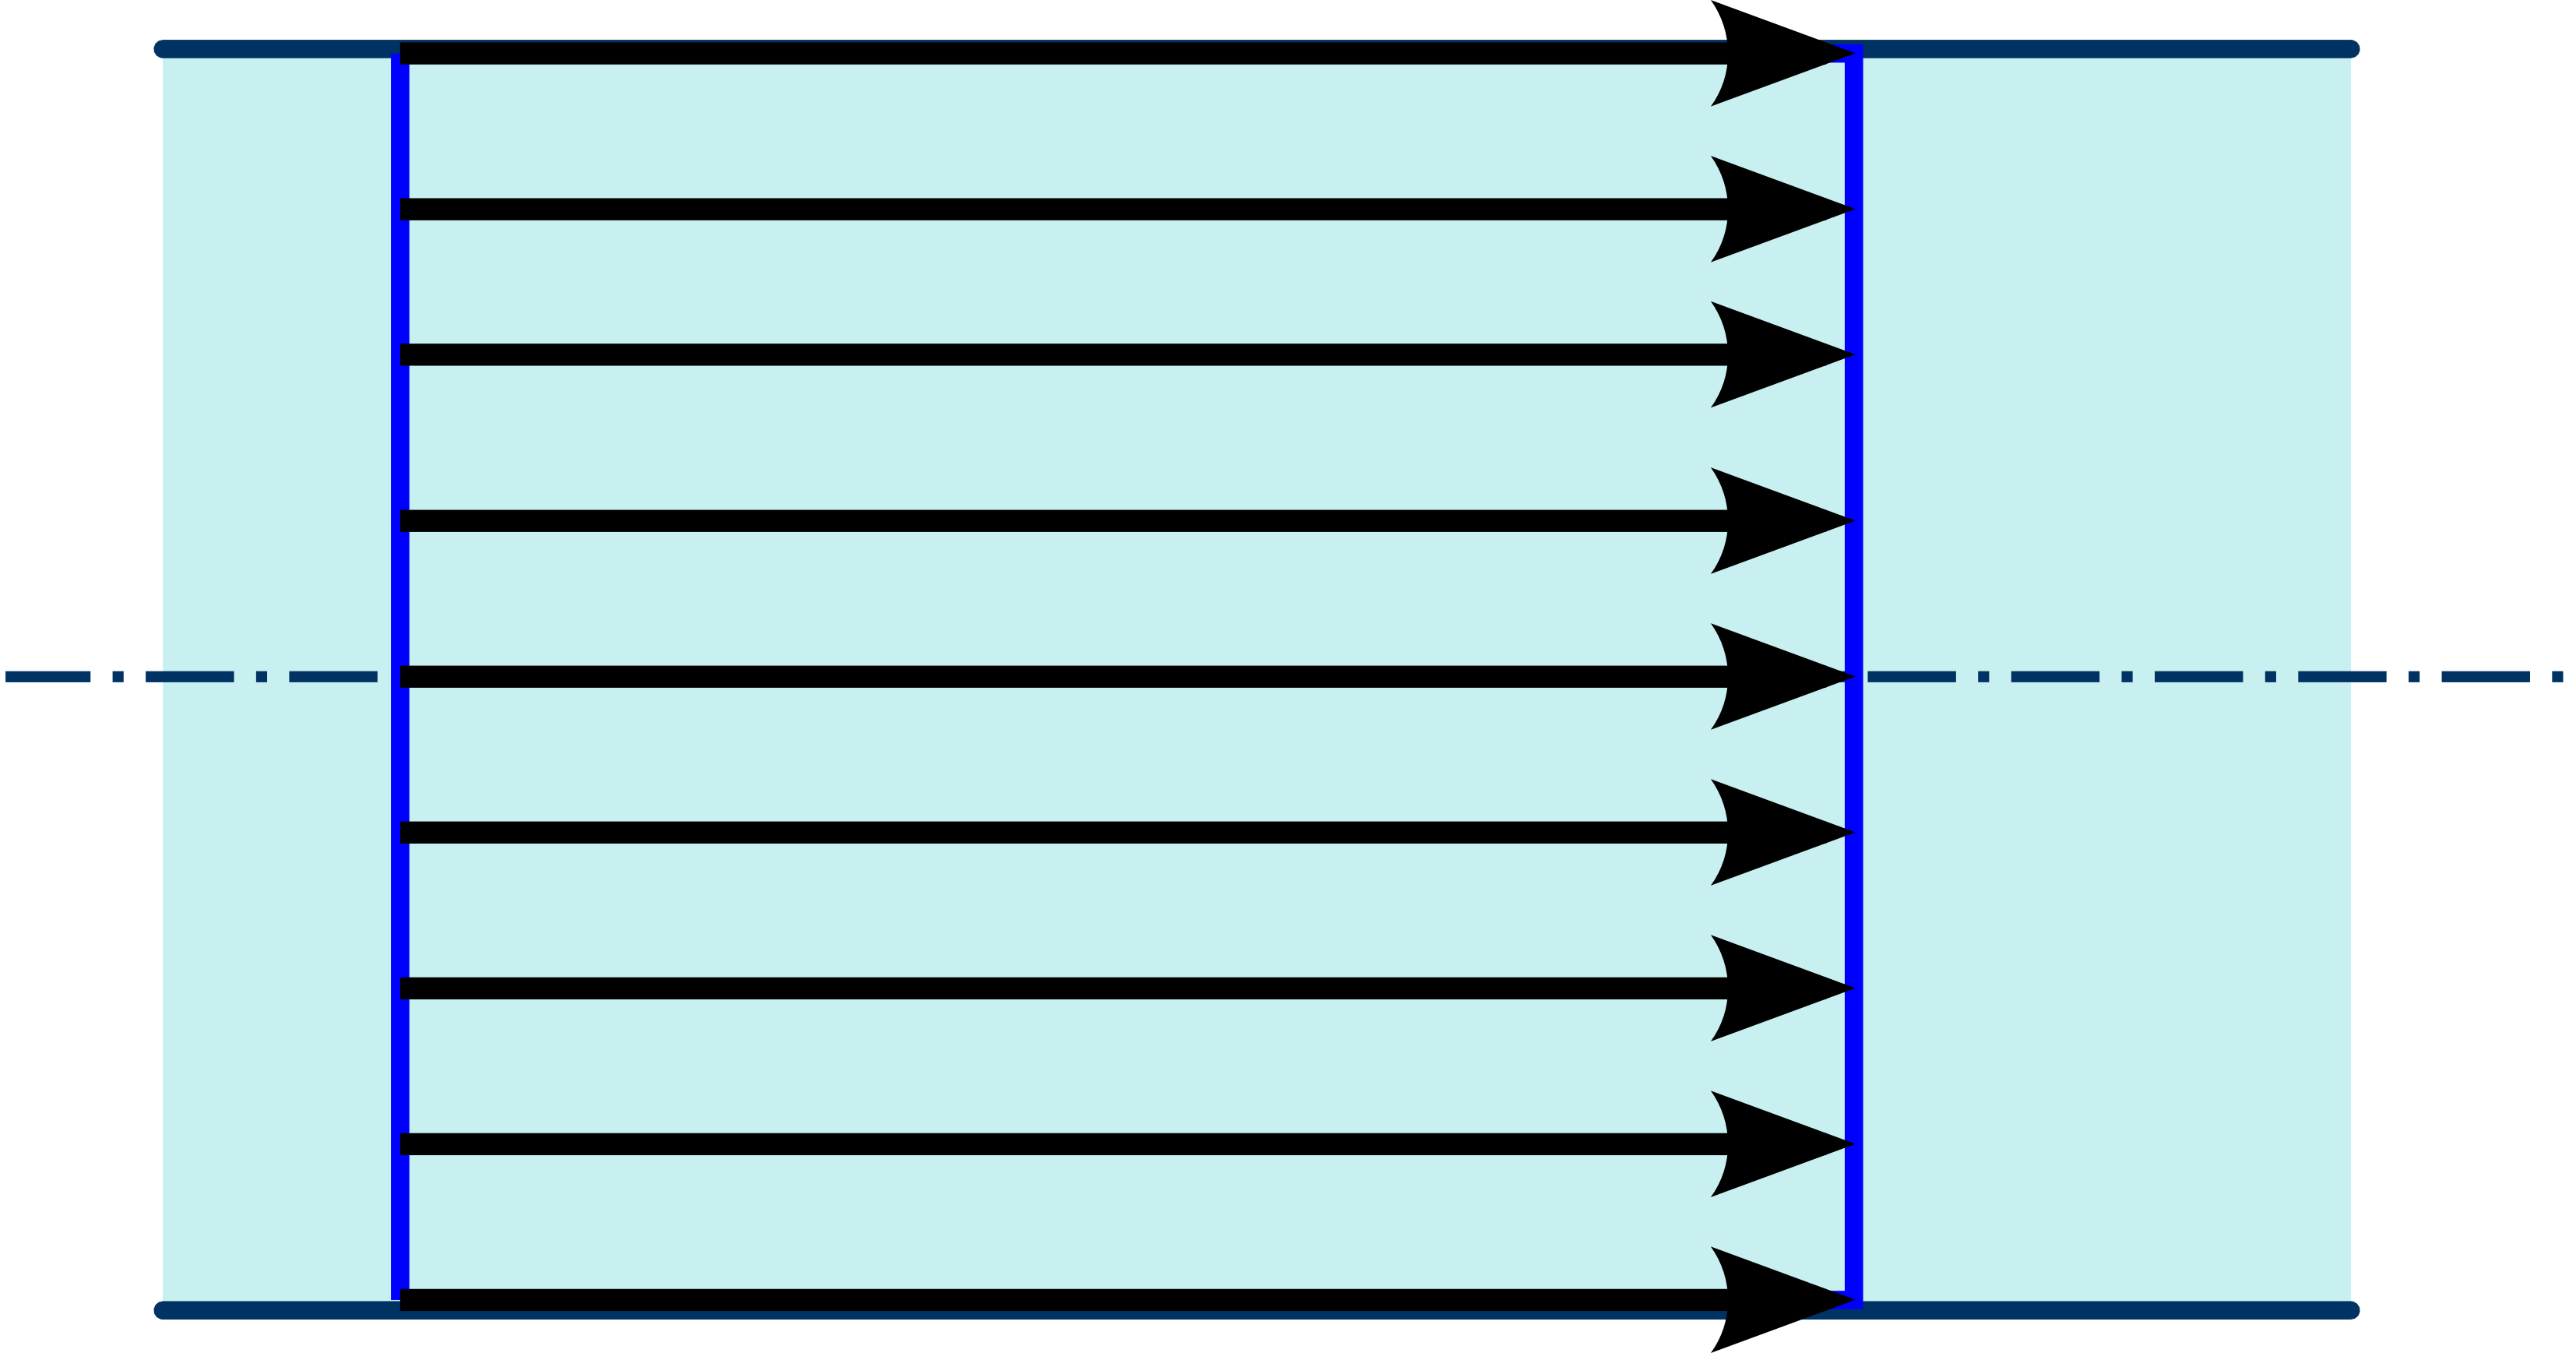
\includegraphics[width=35mm]{profil_turbulent_modele.png}}
%		\put(37, 9.5){\color{bleu} \vector(1, 0){20}}
%		\put(39, 10.5){\color{bleu} modélisation}
%		\put(-2, -3){\color{bleu} Ecoulement turbulent moyen "réel"}
%		\put(58, -3){\color{bleu} Ecoulement turbulent moyen "modèle"}
%		%\put(27, 14){\color{black} $<\!u\!>\!(r)$}
%		\put(87, 14){\color{black} $U$}
%	\end{picture}
%\end{center}
%
%\bigskip
%
%On assimilera donc l'écoulement turbulent dans une conduite à un écoulement moyen stationnaire, de vitesse uniforme dans chaque section correspondant à la vitesse moyenne débitante :
%\[
%	%<\!u\!>\!(r) \quad \rightarrow 
%	\quad \color{rouge} U = \dot m/(\rho S)
%\]
%où $\dot m$ désigne le débit-masse dans la section d'aire $S$.
%
%\vspace{5mm}
%
%\end{frame}

%-----------------------------------------------------------------------------------------
\subsubsection{Volume de contrôle}
%-----------------------------------------------------------------------------------------
\begin{frame}{Volume de contrôle}
%-----------------------------------------------------------------------------------------

\textbf{Hypothèses de base :} fluide homogène et newtonien, écoulement incompressible.


\small

Pour appliquer les bilans intégraux dans la configuration d'une conduite
de paroi fixe et imperméable, considérons le volume de contrôle fixe $\Omega$ associé au tube de courant délimité \\
par la paroi de la conduite :

\begin{center}
	\begin{picture}(80, 33)
		\put(0, 0){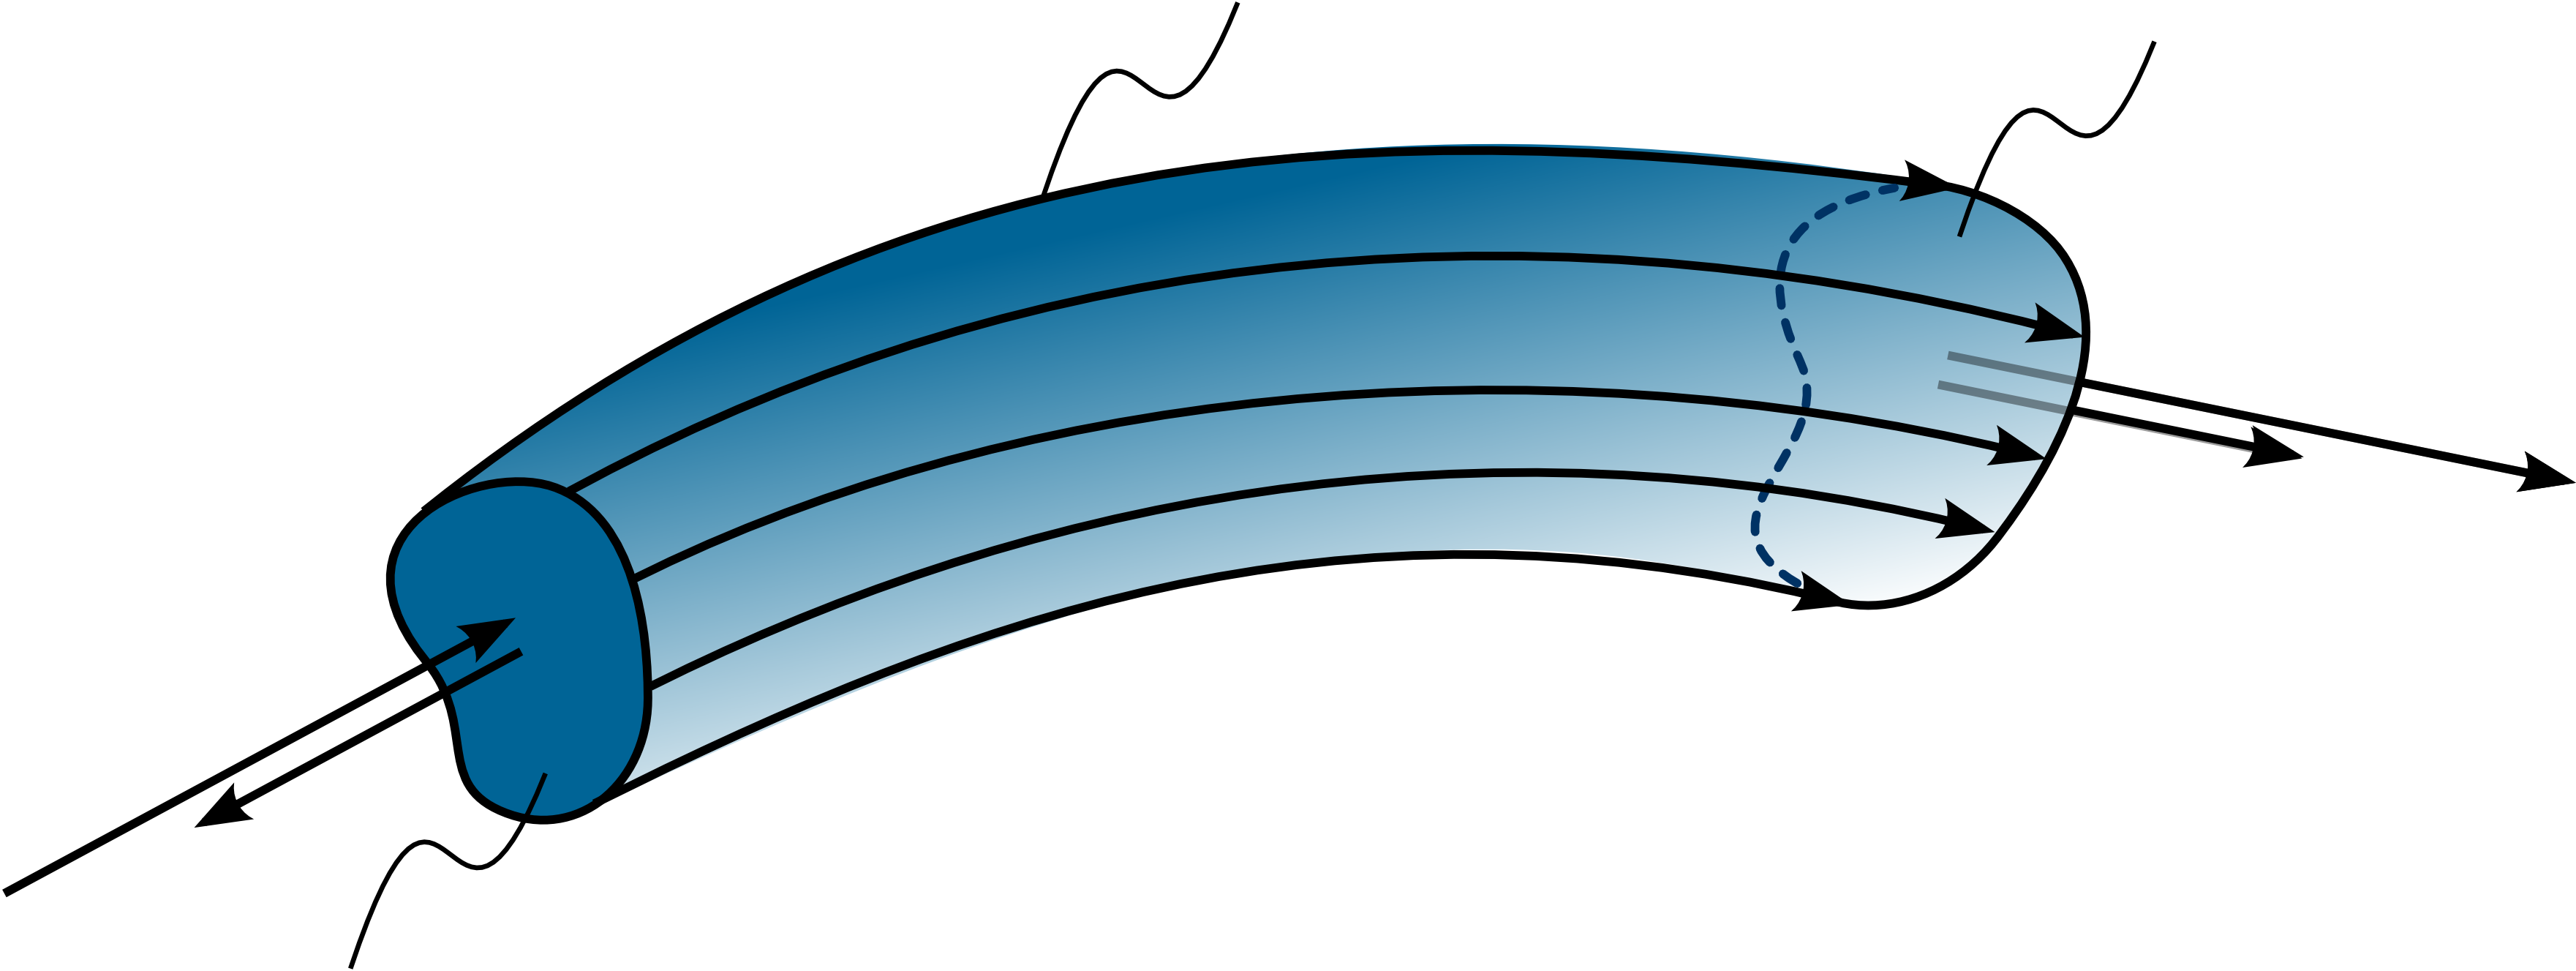
\includegraphics[width=80mm]{streamtube.png}}
		\put(8, -3){$\Gamma_1$ (entrée)}
		\put(5, 1){$\myvec{n}_1$}
		\put(7, 13){$P_1$}
		\put(-6, 9){$\myvec{u}_1 = - U_1 \, \myvec{n}_1$}
		\put(29, 31){$\Sigma$ (paroi) : $\myvec{u}\cdot\myvec{n} = 0$}
		\put(65, 30){$\Gamma_2$ (sortie)}
		\put(66, 13){$\myvec{n}_2$}
		\put(68, 23){$P_2$}
		\put(68, 19){$\myvec{u}_2 = U_2 \, \myvec{n}_2$}
		\put(25, 5){\color{bleu}\vector(1, 0){30}}
		\put(32, 0){\color{bleu} écoulement}
	\end{picture}
\end{center}

\medskip

La frontière du volume de contrôle fixe $\Omega$ est donc donnée par :
\[
	\partial \Omega = \Gamma_1 \cup \Gamma_2 \cup \Sigma
\]
où $\Gamma_1$ et $\Gamma_2$ désignent respectivement les sections d'entrée et de sortie, 
et $\Sigma$ correspond à la surface latérale associée à la paroi. 

\medskip
On rappelle que $\myvec{n}$ désigne la normale sortante à la frontière du volume de contrôle.

\vspace{0mm}

\end{frame}

%-----------------------------------------------------------------------------------------
\subsubsection{Application des bilans intégraux}
%-----------------------------------------------------------------------------------------
\begin{frame}{Application des bilans intégraux}
%-----------------------------------------------------------------------------------------


\small


\textbf{Hypothèses de base :} fluide homogène et newtonien, écoulement incompressible.

\smallskip

%Pour un écoulement turbulent en conduite assimilé à un écoulement moyen 
%quasi uniforme dans chaque section, l'application des bilans intégraux de masse, quantité de mouvement 
%et d'énergie cinétique écrits sur le volume de contrôle précédent permet de montrer que :

\begin{enumerate}
\pause
\item
	le \textcolor{vert}{débit de matière} est conservé :
%	\[
%		\mbox{\color{gris} [Démonstration] \; $\longrightarrow$ \;}

	En terme de débit-masse : $\color{rouge} \dot m = \rho U_1 S_1 = \rho U_2 S_2$
	
	En terme de débit-volume : $\color{orange} Q = U_1 S_1 =  U_2 S_2$
%		\color{rouge} \dot m = \rho U_1 S_1 = \rho U_2 S_2 \quad \mbox{ ou en terme de débit-volume : 
%	\]

Ici $U = \left< u \right>$ est la vitesse normale moyenne dans les sections d'entrée et de sortie.

( $\left< \cdot \right>$  est l'opérateur de moyenne
 sur la section et en temps (dans le cas turbulent).)



\pause
\item
	la \textcolor{vert}{force exercée par l'écoulement sur la conduite} est donnée par
	\[
		\mbox{\color{gris} [Démonstration] \; $\longrightarrow$ \;}
		\color{rouge}
		\myvec{F} = -(P_1+\rho U_1^2) S_1\myvec{n}_1 -(P_2+\rho U_2^2) S_2\myvec{n}_2 + M\myvec{g}
	\]
	où $M$ désigne la masse de fluide contenue dans la portion de conduite entre $S_1$ et $S_2$,

\textcolor{gris}{Application : force exercée sur un tube coudé }%(exo complémentaire Moodle)}


\pause



\item[]
\item
	Le \textcolor{vert}{bilan d'énergie mécanique} entre les sections d'entrée $S_1$
  et de sortie $S_2$ s'écrit :
	\[
		\mbox{\color{gris} [Démonstration] \; $\longrightarrow$ \;}
		\color{rouge}
		Q \left( \bar{e}_{m2} - \bar{e}_{m1} \right) = {\cal P}_{visq,int}	\]
	où :
	
	
	
	1/ 	$
		\bar{e}_m \equiv p + \rho g z 
		+ \dfrac{\alpha}{2} \rho U^2
	$
	correspond à l'énergie mécanique volumique moyenne dans la section concernée; 
	
	2/ $\alpha =  \frac{\left< u^3 \right>}{\left< u \right>^3}$ est un facteur de forme qui vaut 1 pour un écoulement turbulent (profil quasi-uniforme) et 2 pour un écoulement de Poiseuille (démo en exo).
	
	3/   
	${\cal P}_{visq,int} = - \int_\Omega \mytensor{\tau}: \mytensor{D} \, dV =- 2\mu  \int_\Omega \mytensor{D} : \mytensor{D} \, dV \le 0
      $ est la Puissance intérieure des forces visqueuses.

	NB cette loi peut s'interpréter comme une généralisation du (1er) théorème de Bernoulli.
	
	
%\pause
%	\item[]
%	Cette chute d'énergie mécanique est due aux frottements visqueux qui ont lieu à cause du brassage
%	du fluide le long de la conduite : l'énergie mécanique perdue s'est alors transformée en %énergie interne (chaleur).

\end{enumerate}

\vspace{0mm}

\end{frame}

%==========================================================================================
\subsection{Pertes de charge}
%=========================================================================================

%-----------------------------------------------------------------------------------------
\subsubsection{Notion de pertes de charge}
%-----------------------------------------------------------------------------------------
\begin{frame}{Notion de pertes de charge}
%-----------------------------------------------------------------------------------------

Définition : la quantité

\begin{eqnarray*}
\Delta _1^2 &=&  \bar{e}_{m_1} - \bar{e}_{m_2}  \\
               &=& (p_1 + \rho g z_1 
		+ \dfrac{\alpha}{2}\rho U_1^2) -(p_2 + \rho g z_2 
		+ \dfrac{\alpha}{2}\rho U_2^2) \\
	&=& \hat{p_1} - \hat{p_2} \quad (\mbox{ si } S=Cte)
\end{eqnarray*}
	est appelée perte de charge entre les sections 1 et 2.
	
	\medskip
	On a vu la formule explicite :
	$$
	\Delta _1^2 = \frac{-{\cal P}_{visq,int} }{Q} =  \frac{2\mu  \int_\Omega \mytensor{D} : \mytensor{D} \, dV}{Q}
	$$
	
	Cette formule n'est cependant pas utilisable directement (sauf dans le cas laminaire).
	
	\medskip

	Dans le cas général on a recours à l'\textcolor{red}{analyse dimensionnelle} et a des lois approchées issues d'expériences modèles.

\medskip
On distingue : 

-  Pertes de charges 	régulières (proportionnelles à la longueur L du tuyau) 

-  Pertes de charges singulières (dues à des "accidents" localisés).
	
%
%\small
%
%On appellera \textcolor{vert}{pertes de charge}
%entre les sections $S_1$ et $S_2$ la perte d'\'energie 
%m\'ecanique volumique, due \`a la dissipation visqueuse, entre ces deux sections 
%\begin{equation}
%  \Delta _1^2 = \bar{e}_{m_1} - \bar{e}_{m_2} 
%\end{equation}
%
%\medskip
%
%Pour un écoulement turbulent assimilé à un écoulement moyen quasi uniforme,
%\[
%	\bar{e}_m \equiv p + \rho g z + \frac{1}{2}\rho U^2
%\]
%désigne l'énergie mécanique moyenne dans la section concernée.
%
%\medskip
%
%L'\'ecoulement s'effectuant de $S_1$ vers $S_2$ dissipe de l'\'energie m\'ecanique
%par frottement visqueux et par cons\'equent $\Delta _1^2 \ge 0$.
%\medskip
%
%L'\'equation pr\'ec\'edente s'\'ecrit aussi $\bar{e}_{m_1} = \bar{e}_{m_2} + \Delta _1^2$, soit~:
%\begin{equation}
%	\color{rouge}
%  p_1 + \rho g z_1 + \frac{1 }{2} \rho U_1^2 
%  = p_2 + \rho g z_2 + \frac{1 }{2}\rho  U_2^2 + \Delta _1^2
%\end{equation}
%ce qui peut s'interpr\'eter comme une g\'en\'eralisation du th\'eor\`eme de Bernoulli
%(cf. chapitre 7) avec prise en compte de la dissipation visqueuse.
%
%\medskip
%
%L'\'energie m\'ecanique dissip\'ee par frottements visqueux au niveau de la paroi ainsi
%qu'au sein m\^eme du fluide est transform\'ee en \'energie interne dont l'\'evolution 
%est gouvern\'ee par l'\'equation de bilan issue du premier principe de la thermodynamique 
%(cf. cours de transferts thermiques).
%
%\vspace{0mm}

\end{frame}

%-----------------------------------------------------------------------------------------
\subsubsection{Pertes de charge régulières}
%-----------------------------------------------------------------------------------------
\begin{frame}{Pertes de charge régulières}
%-----------------------------------------------------------------------------------------

\small

On appelle \textcolor{vert}{pertes de charge r\'eguli\`eres} (ou \textsl{lin\'eaires}) la diminution
d'\'energie m\'ecanique entre deux sections d'une conduite, \`a parois \'eventuellement rugueuses, de \textsl{section uniforme}.

\begin{center}
  \begin{picture}(85, 28)(0, 5)
     \put(0, 0){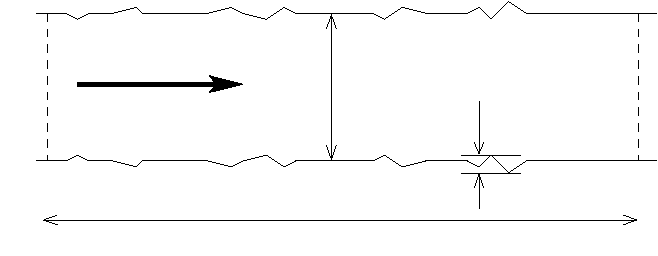
\includegraphics[width=8cm]{conduite.pdf}}
     \put(0, 20){$\hat{p}_1$}
     \put(80, 20){$\hat{p}_2$}
     \put(41, 20){$d$}
     \put(15, 23){$u$}
     \put(15, 17){$\rho, \nu$}
     \put(60, 15){$k$}
     \put(40, 3){\colorbox{white}{$l$}}
  \end{picture}
  
  \bigskip
 \sl Ecoulement dans une conduite rugueuse de section uniforme. \\
  $k$ correspond \`a la taille moyenne des rugosit\'es.
\end{center}

\pause

%Dans ce cas, la conservation du d\'ebit conduit \`a $U_1 = U_2 = U$, vitesse moyenne d\'ebitante dans la conduite, et les pertes de charge s'\'ecrivent, en introduisant la pression motrice $\hat{p} = p + \rho g z$ :
%\begin{equation}
 % \Delta _1^2 
 % = \bar{e}_{m_1} - \bar{e}_{m_2} = \hat{p}_1 - \hat{p}_2 
 % + \frac{1}{2}\rho \left (U_1^2 - U_2^2\right ) = \hat{p}_1 - \hat{p}_2
%\end{equation}
%Les pertes de charge r\'eguli\`eres conduisent alors \`a \textcolor{vert}{une chute de pression motrice} dans la conduite.

Une estimation par analyse dimensionnelle  montre que les pertes de charge r\'eguli\`eres 
ont pour expression {\color{gray} [Démonstration :]}
\begin{equation}
	\color{rouge}
  \Delta _1^2 
             = \frac{1}{2} \, \rho \, U^2 \frac{L}{D} \; \lambda(\varepsilon, Re)
\end{equation}
o\`u l'on d\'efinit $Re = U D/\nu$ et la rugosit\'e relative de la paroi $\varepsilon = k/D$.



$\lambda(\varepsilon, Re)$ est par construction sans dimension et est appel\'e
\textcolor{vert}{coefficient de perte de charge r\'eguli\`eres}.

\vspace{0mm}

\end{frame}

%-----------------------------------------------------------------------------------------
\begin{frame}{Coefficient de pertes de charge}
%-----------------------------------------------------------------------------------------

%$$
%\Delta _1^2  = \frac{1}{2} \, \rho \, U^2 \frac{L}{D} \; \lambda(\varepsilon, Re)
%$$
             

\small

\begin{itemize}

\item Cas laminaire :

Dans ce cas la solution de Poiseuille permet de calculer explicitement la perte de charge et conduit à : $\lambda = 64/Re$ 
{\color{gray}{[Exercice MMC ]}}

On peut retrouver l'ordre de grandeur de ce résultat par analyse dimensionnelle 
{\color{gray}{[Démo]}}

\medskip \pause

\item Cas turbulent "régime très rugueux" :

Si  $\varepsilon > 1\%$ et $Re>10^5$, on observe que la perte de charge est indépendante de Re et donné par la formule approchée (Karman--Nikuradse)
\begin{equation}
   \frac{1}{\sqrt{\lambda}} = -2 \log_{10} \left( \frac{\varepsilon}{3.71} \right)
\end{equation}
\pause 

Paradoxe : $\lambda$ ne dépend plus de $Re$ donc ${\cal P}_{visq,int}$ ne dépend plus de $\mu ???$

Explication : la dissipation est turbulente.

\medskip \pause

\item Cas turbulent, régime "hydroadynamiquement lisse" :

Pour $\varepsilon < 0.01\%$ et $Re<10^5$ on peut utiliser  la formule de Blasius
\begin{equation}
   \lambda= 0.316 \, Re^{-1/4}
   \end{equation}

\medskip \pause

\item Cas turbulent, cas général

Pour $Re >4000$ et $\epsilon$ quelconque, on utilise généralement la formule de 
\textcolor{vert}{Colebrook} (semi-explicite) :
\begin{equation}
	\color{rouge}
  \frac{1}{\sqrt{\lambda}} = -2 \log_{10} \left (
  \frac{2.51}{Re\sqrt{\lambda}} + \frac{\varepsilon}{3.71}
  \right)
\end{equation}

\end{itemize}

%et dans le cas des \'ecoulements dits \textcolor{vert}{hydrauliquement lisses} pour $\varepsilon < 0.01\%$ 
%et $Re<100000$ pour donner la formule de Blasius
%\begin{equation}
  % \lambda= 0.316 \, Re^{-1/4}
%\end{equation}


\medskip \pause

Toutes ces formules sont tabulées dans le diagramme de Moody :


\vspace{0mm}

\end{frame}

%-----------------------------------------------------------------------------------------
\begin{frame}{Diagramme de Moody}
%-----------------------------------------------------------------------------------------

\small

\begin{center}
  \begin{picture}(65, 50)(0, 4)
     \put(0, 2){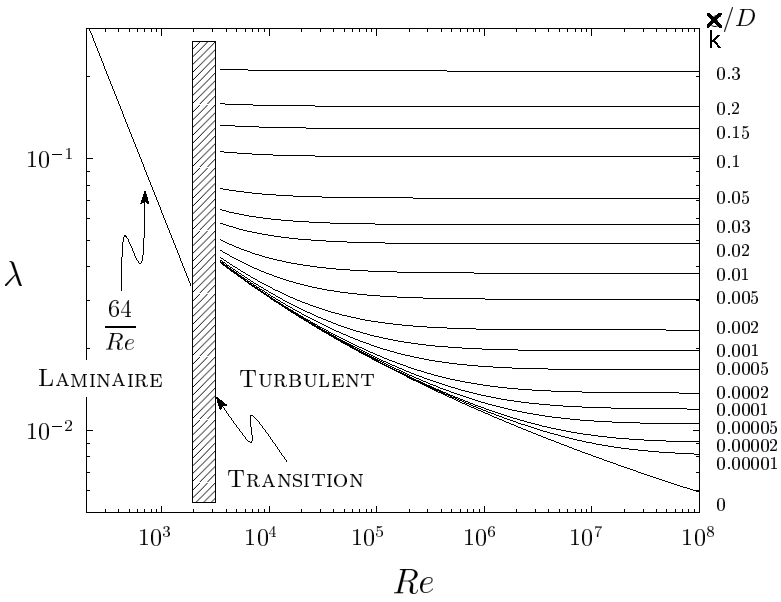
\includegraphics[width=65mm]{Moody_diagram.pdf}}
		\setlength{\fboxsep}{2mm}
     \put(58.5, 49.5){\colorbox{white}{$\varepsilon \quad$}}
		\setlength{\fboxsep}{1mm}
  \end{picture}
\end{center}

\noindent
Le coefficient de pertes de charge r\'eguli\`eres $\lambda$ est donn\'e en fonction du nombre de Reynolds $Re$ 
pour diff\'erentes rugosit\'es relatives $\varepsilon$ dans le \textcolor{vert}{diagramme de Moody} qui est obtenu par 
r\'esolution num\'erique de la formule implicite de Colebrook.


\vspace{5mm}

\end{frame}

%-----------------------------------------------------------------------------------------
\subsubsection{Pertes de charge singulières}
%-----------------------------------------------------------------------------------------
\begin{frame}{Pertes de charge singulières}
%-----------------------------------------------------------------------------------------

\small

On appelle \textcolor{vert}{pertes de charges singuli\`eres} 
la diminution d'\'energie m\'ecanique entre deux sections d'une conduite de part et d'autre d'une \textcolor{vert}{singularit\'e}, c'est-\`a-dire d'une variation \textsl{brusque} de la g\'eom\'etrie de la conduite~:
r\'etr\'ecissement ou \'elargissement brusque, changement de direction (coude) 
ou pr\'esence d'un obstacle.
En effet cette variation brusque des conditions d'\'ecoulement s'accompagne g\'en\'eralement d'une augmentation du brassage du fluide \`a grand nombre de Reynolds et donc des frottements visqueux.


\begin{center}
  \begin{picture}(100, 42)(5, 0)
     \put(0, 0){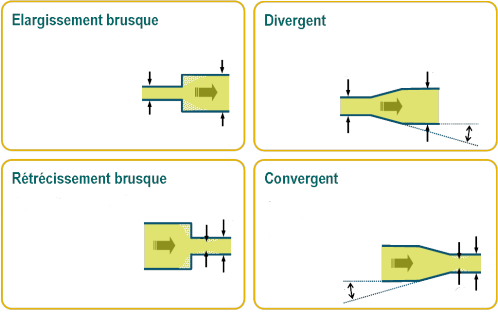
\includegraphics[width=55mm]{pertes_de_charge_singulieres1_naked.png}}
     \put(56, 0.5){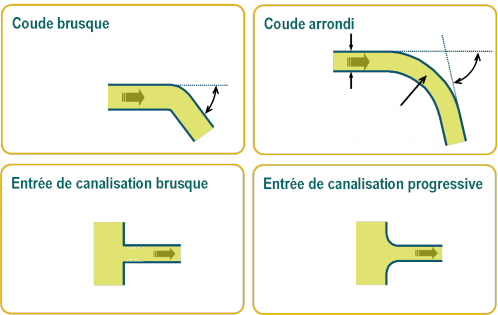
\includegraphics[width=55mm]{pertes_de_charge_singulieres2_naked.png}}
  \end{picture}
\end{center}


\vspace{0mm}

\end{frame}

%-----------------------------------------------------------------------------------------
\begin{frame}{Pertes de charge singulières}
%-----------------------------------------------------------------------------------------

\small

Une estimation par analyse dimensionnelle montre que les pertes de charge singuli\`eres 
s'\'ecrivent
\begin{equation}
	\color{rouge}
  \Delta _1^2 = \frac{1}{2} \, \rho \, u_1^2 \; K
\end{equation}
o\`u $u_1$ est la vitesse moyenne en amont de la singularit\'e et $K$ d\'esigne le \textcolor{vert}{coefficient de pertes de charge singuli\`eres}. 

On observe que pour $Re\gtrsim10^4$ ce coefficient ne dépend pas de $Re$.

Les valeurs de $K$ sont donn\'ees par des formules empiriques ou semi-empiriques en fonction du type de singularit\'e concern\'ee. 

\begin{center}
  \begin{picture}(100, 42)(5, 0)
     \put(0, 0){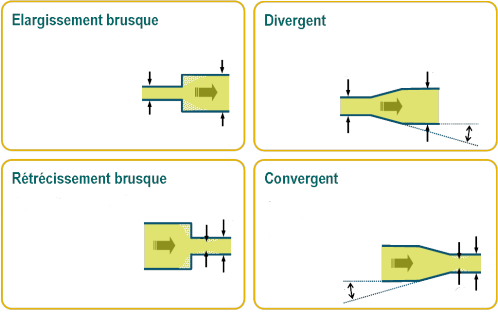
\includegraphics[width=55mm]{pertes_de_charge_singulieres1_naked.png}}
     \put(56, 0.5){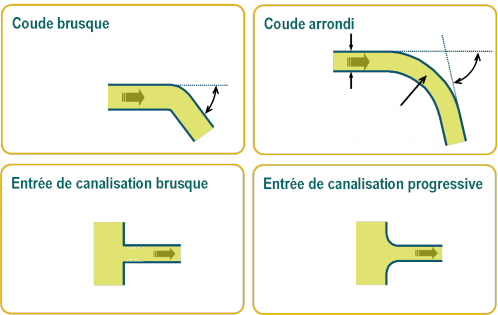
\includegraphics[width=55mm]{pertes_de_charge_singulieres2_naked.png}}

     \put(1, 19.5){\scriptsize $K=(1-S_1/S_2)^2$  \textcolor{vert}{Démo :} }
     \put(15, 28){\scriptsize $S_1$}
     \put(23, 29.1){\scriptsize $S_2$}
     \put(1, 2){\scriptsize $K=(S_2/S_c-1)^2$}
     \put(21, 11){\scriptsize $S_c$}
     \put(23.5, 12){\scriptsize $S_2$}

     \put(29, 29.5){\scriptsize $K=(1-S_1/S_2)^2 \sin \alpha$}
     \put(35, 19.5){\scriptsize $S_1$}
     \put(43.5, 19.5){\scriptsize $S_2$}
     \put(52.5, 19.5){\scriptsize $\alpha$}
     \put(29, 12){\scriptsize $K=(S_2/S_c-1)^2 \sin \alpha$}
     \put(49, 9){\scriptsize $S_c$}
     \put(51.5, 10){\scriptsize $S_2$}
     \put(36, 2){\scriptsize $\alpha$}

     \put(57, 29.5){\scriptsize $K=\sin^2 \alpha + 2\sin^4 \alpha/2$}
     \put(80, 23){\scriptsize $\alpha$}
     \put(57, 12){\scriptsize $K = 0.5$}
     
     \put(85, 23){\scriptsize $K= \dfrac{\alpha}{\pi} \big [0.131 $}
     \put(85, 19.2){\scriptsize $+ 1.847 (D/R)^{7/2}\big]$}
     \put(90, 28){\scriptsize $D$}
     \put(99, 25){\scriptsize $R$}
     \put(108, 26){\scriptsize $\alpha$}
     \put(85, 12){\scriptsize $K = 0.04$}
     
  \end{picture}
\end{center}

Quelques éléments de plomberie standard :

Raccord rectiligne $K = 0.04$ ;  Valve "globe" ouverte $K = 6.4$ ; valve demi-fermée $K = 9.5$ ; 

Coude $90^o$ standard $K= 0.75$ ; coude à grand rayon $K = 0.45$ ;

Raccord en $T$ $K = 0.4$ (ligne$\rightarrow$ligne) / $K=1.3$ 
(ligne$\rightarrow$branche) / $K=1.5$ (branche$\rightarrow$ligne)....

\vspace{0mm}

\end{frame}
\comment{
\begin{frame}{Applications}
\small

Applications :

\medskip 
Exemple 1 : dimensionnement d'un chauffe-eau solaire.

\medskip
Exemple 2 : canalisation en pente.


\end{frame}
}

%%%%%%%%%%%%%%%%%%%%%%%%%%%%%%%%%%%%%%%%%%%%%%%%%%%%%%%%%%%%%%%%%%%%%%%%%%%%%%%%%%%%%%%%%%%
\comment{
%%%%%%%%%%%%%%%%%%%%%%%%%%%%%%%%%%%%%%%%%%%%%%%%%%%%%%%%%%%%%%%%%%%%%%%%%%%%%%%%%%%%%%%%%%%

%==========================================================================================
\subsection*{Compléments}
%==========================================================================================

%------------------------------------------------------------------------------------------
\begin{frame}{toto} \hypertarget{frame:toto}{}
%------------------------------------------------------------------------------------------

\small

\vspace{0mm}

\end{frame}
}

